% DON'T FORGET TO ADD YOUR OWN NAME AND TITLE in the "hyperref" package
% configuration below. THIS INFORMATION GETS EMBEDDED IN THE PDF FINAL PDF DOCUMENT.
% You can view the information if you view Properties of the PDF document.

% -----------------------------------------------------------------------

% By default, output is produced that is geared toward generating a PDF 
% version optimized for viewing on an electronic display, including 
% hyperlinks within the PDF.

% To create a PDF output that is optimized for double-sided printing: 
%
% 1) comment-out the \documentclass statement in the preamble below, and
% un-comment the second \documentclass line.
%
% 2) change the value assigned below to the boolean variable
% "PrintVersion" from "false" to "true".

% --------------------- Start of Document Preamble -----------------------

% Specify the document class, default style attributes, and page dimensions
% For hyperlinked PDF, suitable for viewing on a computer, use this:
\documentclass[letterpaper,12pt,titlepage,oneside,final]{book}
 
% For PDF, suitable for double-sided printing, change the PrintVersion variable below
% to "true" and use this \documentclass line instead of the one above:
%\documentclass[letterpaper,12pt,titlepage,openright,twoside,final]{book}

% Some LaTeX commands I define for my own nomenclature.
% If you have to, it's better to change nomenclature once here than in a 
% million places throughout your thesis!
\newcommand{\package}[1]{\textbf{#1}} % package names in bold text
\newcommand{\cmmd}[1]{\textbackslash\texttt{#1}} % command name in tt  
\newcommand{\href}[1]{#1} % does nothing, but defines the command so the
    % print-optimized version will ignore \href tags (redefined by hyperref pkg).
%\newcommand{\texorpdfstring}[2]{#1} % does nothing, but defines the command
% Anything defined here may be redefined by packages added below...

% This package allows if-then-else control structures.
\usepackage{ifthen}
\newboolean{PrintVersion}
\setboolean{PrintVersion}{false} 
% CHANGE THIS VALUE TO "true" as necessary, to improve printed results for hard copies
% by overriding some options of the hyperref package below.

%\usepackage{nomencl} % For a nomenclature (optional; available from ctan.org)
\usepackage{amsmath,amssymb,amstext} % Lots of math symbols and environments
\usepackage[pdftex]{graphicx} % For including graphics N.B. pdftex graphics driver 
%change this to the folder with all of your gifures
\graphicspath{ {figures/} }

% si units
\usepackage{siunitx}
% bigints allows for much larger integral signs. Useful for integrals with nested fractions.
\usepackage{bigints}
% float allows you to place a figure at precisely the location in the LaTeX code. 
\usepackage{float}
% "This makes your tables nicer" - Dimuth
\usepackage{booktabs}
\setlength\heavyrulewidth{.35ex}

\usepackage{times}

\usepackage{subcaption}

\usepackage{float}

\usepackage{natbib}

\usepackage{fancyhdr}

%\usepackage[square,numbers,sectionbib]{natbib}
\usepackage{chapterbib}

% Hyperlinks make it very easy to navigate an electronic document.
% In addition, this is where you should specify the thesis title
% and author as they appear in the properties of the PDF document.
% Use the "hyperref" package 
% N.B. HYPERREF MUST BE THE LAST PACKAGE LOADED; ADD ADDITIONAL PKGS ABOVE
\usepackage[pdftex,pagebackref=false]{hyperref} % with basic options
		% N.B. pagebackref=true provides links back from the References to the body text. This can cause trouble for printing.
\hypersetup{
    plainpages=false,       % needed if Roman numbers in frontpages
    unicode=false,          % non-Latin characters in Acrobat’s bookmarks
    pdftoolbar=true,        % show Acrobat’s toolbar?
    pdfmenubar=true,        % show Acrobat’s menu?
    pdffitwindow=false,     % window fit to page when opened
    pdfstartview={FitH},    % fits the width of the page to the window
    pdftitle={Title},    % title: CHANGE THIS TEXT!
    pdfauthor={Michael A. Allen},    % author: CHANGE THIS TEXT! and uncomment this line
%    pdfsubject={Subject},  % subject: CHANGE THIS TEXT! and uncomment this line
%    pdfkeywords={keyword1} {key2} {key3}, % list of keywords, and uncomment this line if desired
    pdfnewwindow=true,      % links in new window
    colorlinks=true,        % false: boxed links; true: colored links
    linkcolor=blue,         % color of internal links
    citecolor=green,        % color of links to bibliography
    filecolor=magenta,      % color of file links
    urlcolor=cyan           % color of external links
}
\ifthenelse{\boolean{PrintVersion}}{   % for improved print quality, change some hyperref options
\hypersetup{	% override some previously defined hyperref options
%    colorlinks,%
    citecolor=black,%
    filecolor=black,%
    linkcolor=black,%
    urlcolor=black}
}{} % end of ifthenelse (no else)

\usepackage[automake,toc,abbreviations]{glossaries-extra} % Exception to the rule of hyperref being the last add-on package

% Setting up the page margins...
\setlength{\marginparwidth}{0pt} % width of margin notes
% N.B. If margin notes are used, you must adjust \textwidth, \marginparwidth
% and \marginparsep so that the space left between the margin notes and page
% edge is less than 15 mm (0.6 in.)
\setlength{\marginparsep}{0pt} % width of space between body text and margin notes
\setlength{\evensidemargin}{0.125in} % Adds 1/8 in. to binding side of all 
% even-numbered pages when the "twoside" printing option is selected
\setlength{\oddsidemargin}{0.125in} % Adds 1/8 in. to the left of all pages
% when "oneside" printing is selected, and to the left of all odd-numbered
% pages when "twoside" printing is selected
\setlength{\textwidth}{6.375in} % assuming US letter paper (8.5 in. x 11 in.) and 
% side margins as above
\raggedbottom

% The following statement specifies the amount of space between
% paragraphs. Other reasonable specifications are \bigskipamount and \smallskipamount.
\setlength{\parskip}{\medskipamount}

% The following statements controls the line spacing, baselinestrech is default. setspace only 
% controls spacing in the body/bibliogoraphy and leaves the rest defaulted.
%\renewcommand{\baselinestretch}{1.2} 
\usepackage{setspace}
\setstretch{1.5}

%indents the first line of each paragraph
\usepackage{indentfirst}


% By default, each chapter will start on a recto (right-hand side)
% page.  We also force each section of the front pages to start on 
% a recto page by inserting \cleardoublepage commands.
% In many cases, this will require that the verso page be
% blank and, while it should be counted, a page number should not be
% printed.  The following statements ensure a page number is not
% printed on an otherwise blank verso page.
\let\origdoublepage\cleardoublepage
\newcommand{\clearemptydoublepage}{%
  \clearpage{\pagestyle{empty}\origdoublepage}}
\let\cleardoublepage\clearemptydoublepage



% Define Glossary terms (This is properly done here, in the preamble. Could be \input{} from a file...)
% Main glossary entries -- definitions of relevant terminology
\newglossaryentry{computer}
{
name=computer,
description={A programmable machine that receives input data,
               stores and manipulates the data, and provides
               formatted output}
}
\newglossaryentry{waveband}
{
	name=waveband,
	description={The range of wavelengths in between upper and lower 
		bounds. Usually refers to the spectral range over which 
		a sensor responds.}
}
\newglossaryentry{uhi}
{
	name=urban heat island effect,
	description={The tendency for cities to store and emit a greater amount of heat compared to non---urbanized surroundings. Generally manifests in elevated urban air and surface temperatures.}
}
\newglossaryentry{atmwind}
{
	name=atmospheric window,
	description={A region of the electromagnetic spectrum over which the atmosphere is transmissive. Two are located in the thermal infrared \gls{waveband} at approximately 3 - 5 and 8 - 14\SI{}{\micro\metre}.}
}
\newglossaryentry{pyrg}
{name={pyrgeometer},
	description={description}
}
\newglossaryentry{fov}
{name={field-of-view},
	description={description}
}
\newglossaryentry{blayer}{
	name={boundary-layer},
	description={description}
}

% List of Abbreviations (abbreviations type is built in to the glossaries-extra package)
\newabbreviation{aaaaz}{AAAAZ}{American Association of Amature Astronomers and Zoologists}

% List of Symbols
\newglossary*{symbols}{List of Symbols}
\newglossaryentry{rvec}
{
name={$\mathbf{v}$},
sort={label},
type=symbols,
description={Random vector: a location in n-dimensional Cartesian space, where each dimensional component is determined by a random process}
}
 
\makeglossaries

%======================================================================
%   L O G I C A L    D O C U M E N T -- the content of your thesis
%======================================================================
\begin{document}
\raggedright
\setlength{\parindent}{6ex}


% For a large document, it is a good idea to divide your thesis
% into several files, each one containing one chapter.
% To illustrate this idea, the "front pages" (i.e., title page,
% declaration, borrowers' page, abstract, acknowledgements,
% dedication, table of contents, list of tables, list of figures,
% nomenclature) are contained within the file "uw-ethesis-frontpgs.tex" which is
% included into the document by the following statement.
%----------------------------------------------------------------------
% FRONT MATERIAL
%----------------------------------------------------------------------
% T I T L E   P A G E
% -------------------
% Last updated Nov 1, 2016, by Stephen Carr, IST-Client Services
% The title page is counted as page `i' but we need to suppress the
% page number.  We also don't want any headers or footers.
\pagestyle{empty}
\pagenumbering{roman}

% The contents of the title page are specified in the "titlepage"
% environment.
\begin{titlepage}
        \begin{center}
        \vspace*{1.0cm}

        \Huge
        {\bf A Method to Assess the Surface Urban Heat Island Effect Using Hemispherical Radiometric Surface Temperatures}

        \vspace*{1.0cm}

        \normalsize
        by \\

        \vspace*{1.0cm}

        \Large
        Michael A. Allen \\

        \vspace*{3.0cm}

        \normalsize
        A thesis \\
        presented to the University of Western Ontario\\ 
        in fulfillment of the \\
        thesis requirement for the degree of \\
        Master of Science \\

        \vspace*{2.0cm}

        London, Ontario, Canada, 2017 \\

        \vspace*{1.0cm}

        \copyright\ Michael A. Allen 2017 \\
        \end{center}
\end{titlepage}

% The rest of the front pages should contain no headers and be numbered using Roman numerals starting with `ii'
\pagestyle{plain}
\setcounter{page}{2}

\cleardoublepage % Ends the current page and causes all figures and tables that have so far appeared in the input to be printed.
% In a two-sided printing style, it also makes the next page a right-hand (odd-numbered) page, producing a blank page if necessary.
 


% D E C L A R A T I O N   P A G E
% -------------------------------
  % The following is a sample Delaration Page as provided by the GSO
  % December 13th, 2006.  It is designed for an electronic thesis.
  \noindent
I hereby declare that I am the sole author of this thesis. This is a true copy of the thesis, including any required final revisions, as accepted by my examiners.

  \bigskip
  
  \noindent
I understand that my thesis may be made electronically available to the public.

\cleardoublepage

% A B S T R A C T
% ---------------

\begin{center}\textbf{Abstract}\end{center}

This is the abstract.



\cleardoublepage

% A C K N O W L E D G E M E N T S
% -------------------------------

\begin{center}\textbf{Acknowledgments}\end{center}

These are my Acknowledgments
\cleardoublepage

% T A B L E   O F   C O N T E N T S
% ---------------------------------
\renewcommand\contentsname{Table of Contents}
\tableofcontents
\cleardoublepage
\phantomsection    % allows hyperref to link to the correct page

% L I S T   O F   T A B L E S
% ---------------------------
\addcontentsline{toc}{chapter}{List of Tables}
\listoftables
\cleardoublepage
\phantomsection		% allows hyperref to link to the correct page

% L I S T   O F   F I G U R E S
% -----------------------------
\addcontentsline{toc}{chapter}{List of Figures}
\listoffigures
\cleardoublepage
\phantomsection		% allows hyperref to link to the correct page

% GLOSSARIES (Lists of definitions, abbreviations, symbols, etc. provided by the glossaries-extra package)
% -----------------------------
\printglossaries
\cleardoublepage
\phantomsection		% allows hyperref to link to the correct page

% Change page numbering back to Arabic numerals and have it in the upper right corner
\pagenumbering{arabic}
\renewcommand{\headrulewidth}{0pt}
\pagestyle{fancy}
\fancyhf{}
\rhead{\thepage}

 

%----------------------------------------------------------------------
% MAIN BODY
%----------------------------------------------------------------------
% Because this is a short document, and to reduce the number of files
% needed for this template, the chapters are not separate
% documents as suggested above, but you get the idea. If they were
% separate documents, they would each start with the \chapter command, i.e, 
% do not contain \documentclass or \begin{document} and \end{document} commands.

\begin{bibunit}
	
\rhead{\thepage}

\chapter{Introduction}
Urban development drastically changes the character of the surface. Replacement of natural terrain with roads, buildings, parks, and other urban features modifies the geometry of the surface as well as its thermal, radiative, moisture, and aerodynamic properties. These modifications, combined with anthropogenic emissions of heat, result in a distinct urban climate; one which is often warmer, a phenomenon termed the urban heat island effect (UHI). As both the Earth's population and the urbanized fraction of that population increase \citep{Nations2014}, cities grow and more people are exposed to urban-modified atmospheres. Thus, understanding how cities interact with the climate across spatiotemporal scales has important implications for human health, energy efficiency, and for informing future urban development. This, in part, has prompted significant expansion in study of the urban effect on climates, particularly in the decades preceding this thesis. 

The notion that urban areas have elevated air and surface temperatures (T\textsubscript{air} and T\textsubscript{surf} respectively) is not new, with the first formal studies of the urban effect on T\textsubscript{air} dating back to \citet{Howard1833}'s identification of "artificial warming" and "urban contamination" in his characterization of spatial patterns of T\textsubscript{air} in early 19\textsuperscript{th} century London. Conceptually, contemporary studies of urban climate do not stray far from \citet{Howard1833}, by seeking to isolate and quantify the urban signal in measured or modeled assessment of a given meteorological variable. However, as \citet{Howard1833} identified nearly two centuries ago, the sheer number of factors influencing direct measurement of climates makes experimental control nearly impossible in observational study. In any given observation of climate, myriad urban and non urban signals make it difficult to determine what is urban and what is not, degrading interstudy comparison. Even in the modeling domain, where experimental control is possible, the inherent complexity in simulating flows of energy, momentum, and mass at the scales necessary to represent physical phenomena over realistic urban environments is, as of yet, not possible. Notwithstanding implementation of accurate, physically based schemes to represent urban climates in regional or global climate models. Thus, accurate assessment how a city affects the climate is a deceptively challenging task. To address this, \citet{Lowry1977} presents a framework to isolate the urban effect in observation of a given meteorological variable. In his framework - termed the "Lowry method" - measurement of a meteorological variable ($V_M$) is the sum of forcings from the background climate and synoptic conditions ($V_B$), local topography ($V_L$), and the urban landscape ($V_H$)

\begin{equation}
	V_M = V_B + V_L + V_H
\end{equation}

Thus, isolation of the urban effect on observed $V_M$ simply requires the removal of $V_B$ and $V_L$. This can be achieved by subtracting some urban affected observation ($V_{M, U}$) from a non-urban observation ($V_{M, R}$) where $V_{H, R}$ = 0,

\begin{equation}
V_{M, U} - V_{M, R} = (V_B + V_L + V_H) - (V_B + V_L) = V_H
\end{equation}

\noindent simplified as,

\begin{equation}
	V_H = V_{M, U} - V_{M, R}
\end{equation}

Study of the urban heat island effect tacitly falls into such a framework, by replacing $V_{M, U} - V_{M, R}$ with $\Delta$T\textsubscript{air, U-R}. However, in spite of its conceptual simplicity through the lens of the Lowry method, meta-analysis of observational air temperature UHI (aUHI) study suggests that that simplicty may not translate well to real world analysis. In his analysis of the aUHI literature, \citet{Stewart2011} found that nearly fifty percent of aUHI studies published between 1950 and 2007 are "scientifically indefensible" based on an analysis of relevant criteria\footnote{Each study was given a "passing" or "failing" grade and ranked using a points-based scheme to assess methodological quality in the following criteria: conceptual model, operational definitions, instrument specification, site metadata, site representativeness, number of replicates, weather control, surface control, and synchronicity.}, suggesting a significant gulf between conceptual simplicity and practical realities in aUHI analysis. Of the 190 surveyed studies, only 13\% were derived from field sites that were sufficiently representative of the local-scale environment or lacked the meta-data to make such a determination, leading to potential biases from micro-scale terrain. This is particularly discouraging as it is not the result of an evolution in measurement techniques or improved instrumentation, as techniques to observe and analyze aUHI did not see significant evolution since 1950 - in fact, \citet{Stewart2011} suggests the opposite: a disproportionately large number of studies deemed scientifically sound were published early in the study purview. Thus, in study of the urban effect on variables for which significant methodological shifts have or will occur, the warnings implicit in \citet{Stewart2011} are particularly salient, as inherent difficulties found in translating "Lowry"-esque conceptual models to real world observations may be compounded by significant methodological changes. In the five years since its publication, aUHI study has seen further expansion and, as such, it is difficult to assess whether its critical analysis has prompted a shift towards more thoughtful, careful, and methodical study of aUHI, notwithstanding its relevance in study of the urban effect on different meteorological variables.

In contrast to study of urban T\textsubscript{air}, the introduction of new methods, instruments, and analytical techniques in TIR remote sensing of urban environments has lead to rapid evolution in study of the urban effect on land T\textsubscript{surf} - a vast majority of which has focused on passive remote sensing of upwelling TIR. In the decades preceding this thesis, a combination of factors has lead to an increased focus on remote sensed study of urban T\textsubscript{surf}: 

\begin{itemize}
	\item The proliferation of satellite and aerial thermal infrared (TIR) remote sensors and "openness" in data access policies.
	\item Improvements in sensor spatial, spatial, and radiometric resolutions. 
	\item An increased focus on the importance of the surface in both determining and understanding key near-ground micro-meteorological phenomena.
\end{itemize}

Remote sensed study of the urban effect on land T\textsubscript{surf} has been instrumental in characterizing large-scale spatial and temporal patterns of sUHI \citep{Peng2012, Streutker2003, Imhoff2010}. However, the methodological and conceptual concerns raised in \citet{Stewart2011} in combination with the wide (and broadening) range of methodologies for remote sensed urban T\textsubscript{surf} retrieval should prompt critical assessment of the remote sensed sUHI literature. Difficulties suggested in \citet{Stewart2011} may be amplified by methodological shifts and a variety of methods for analysis. At the time of writing, no systemic or critical reviews of the remote sensed sUHI literature are available. An increasingly dogmatic focus on improving spatial and radiometric resolutions has left other inherent biases in remote sensing of urban environments largely ignored in sUHI literature. This suggests that similar conclusions to those found of aUHI literature in \citet{Stewart2011} are possible (if not likely) for study of sUHI. 

Traditional methods for urban T\textsubscript{surf} measurement are subject to a suite of geometric and temporal biases. These biases are largely inherent to the discipline and contribute an additional source of error on top of potential concerns carried over from meta-analysis of conceptual flaws in aUHI literature. 

Geometric biases in TIR remote sensing of the urban surface are the result of urban modification of surface structure and thermal and radiative properties. Relative to typical non-urban and rural terrain, urban development adds significant 3-dimensionality to the surface. This added complexity results in undersampling of the surface by narrow-FOV remote sensors. A narrow-FOV sensor, by sampling surface 3-dimensionality in 2-dimensions, "sees" a different assemblage of urban surfaces depending on its viewing direction, resulting in a geometric bias towards some arrangement of facets. I.e. viewing from the nadir, a narrow-FOV sensor sees the urban surface as an array of rooftops and roads, the same sensor viewing the from an oblique angle sees some array of walls, rooftops, and roads depending on its orientation. For a sensor in the nadir, increasing FOV introduces sampling of vertical features. To illustrate how sensor-surface geometry influences sampling of the urban surface by narrow- and wide-FOV sensors, Figure \ref{model} shows FOVs for the three sensor orientation/type combinations.The vast majority of urban thermal remote sensing is done via a narrow-FOV sensor in the nadir.

\begin{figure}[H]
	\centering
	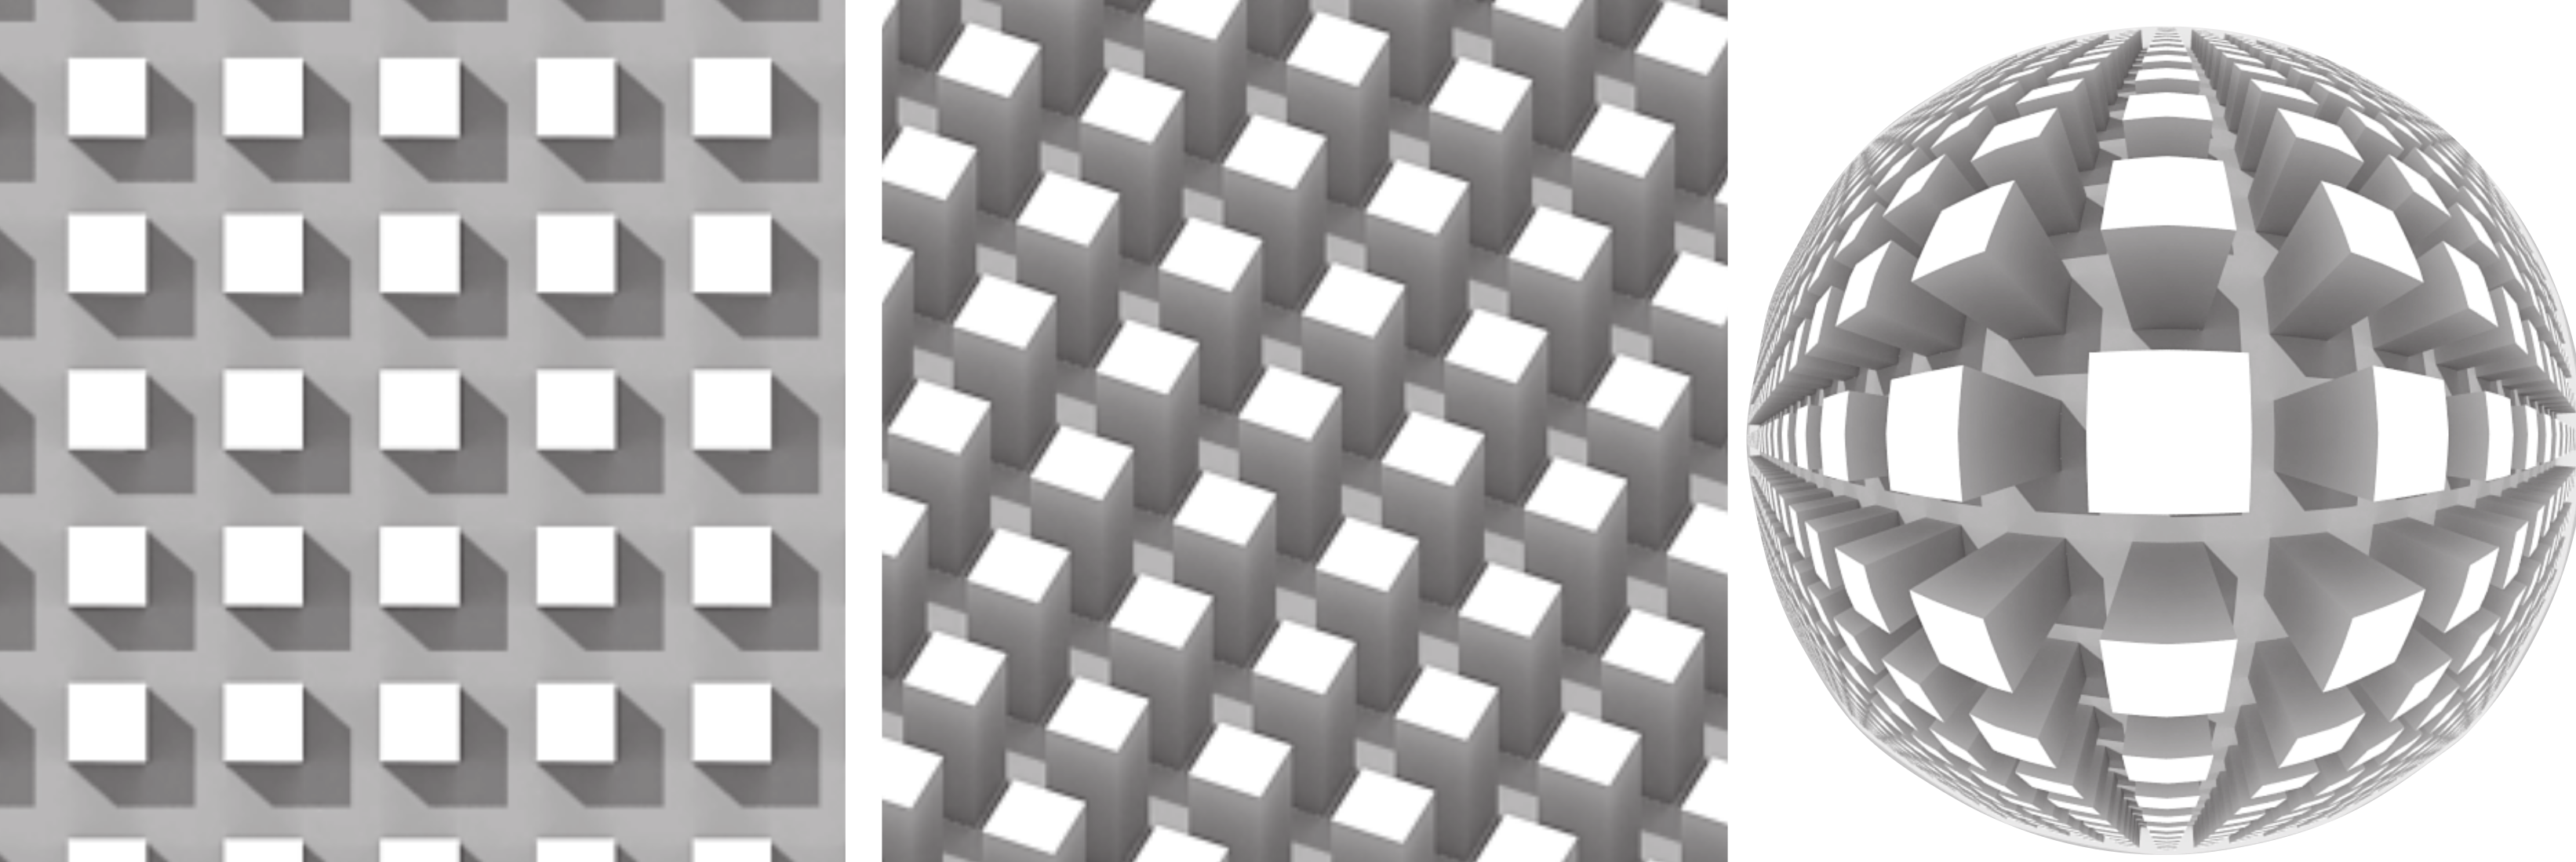
\includegraphics[width=15cm,
	height=7in,
	keepaspectratio]{model}
	\caption{Projected FOVs for a narrow-FOV sensor at nadir and oblique angles, and a wide-FOV hemispherical sensor viewing an idealized urban array with building width T\textit{H}, height 2\textit{H}, and inter element spacing textit{H}. Figure from \cite{Adderley2015}.}
	\label{model}
\end{figure}


In addition to modifying how a remote sensor samples the surface, the convoluted 3-dimensional structure of the urban surface modifies sunlit/shading regimes, resulting in strong micro-scale spatiotemporal contrasts in urban T\textsubscript{surf}, which depend on surface-sun geometry. These microscale variations in urban T\textsubscript{surf} are often amplified by significant directional contrasts in the thermal admittance of common urban materials, which determines the diurnal amplitude of T\textsubscript{surf} for a given facet. Thus, when viewed from a narrow-FOV remote sensor with some inherent geometric bias, urban T\textsubscript{surf} is directionally dependent - constituting an "effective anisotropy" of urban T\textsubscript{surf}, shown in Figure \ref{anisot}. The qualifier "effective" is used to differentiate directional contrasts in urban T\textsubscript{surf} that arise from a city's 3-dimensional surface structure from those resulting from the non-Lambertian nature of individual urban facets (e.g. walls, rooftops, or roads). The magnitude of urban effective anisotropy can reach up to 10 \si{\kelvin} and is highly dependent on surface-sensor-sun geometry, surface structure, and urban materials \citep{Krayenhoff2016, Voogt1997}. 

\begin{figure}[H]
	\centering
	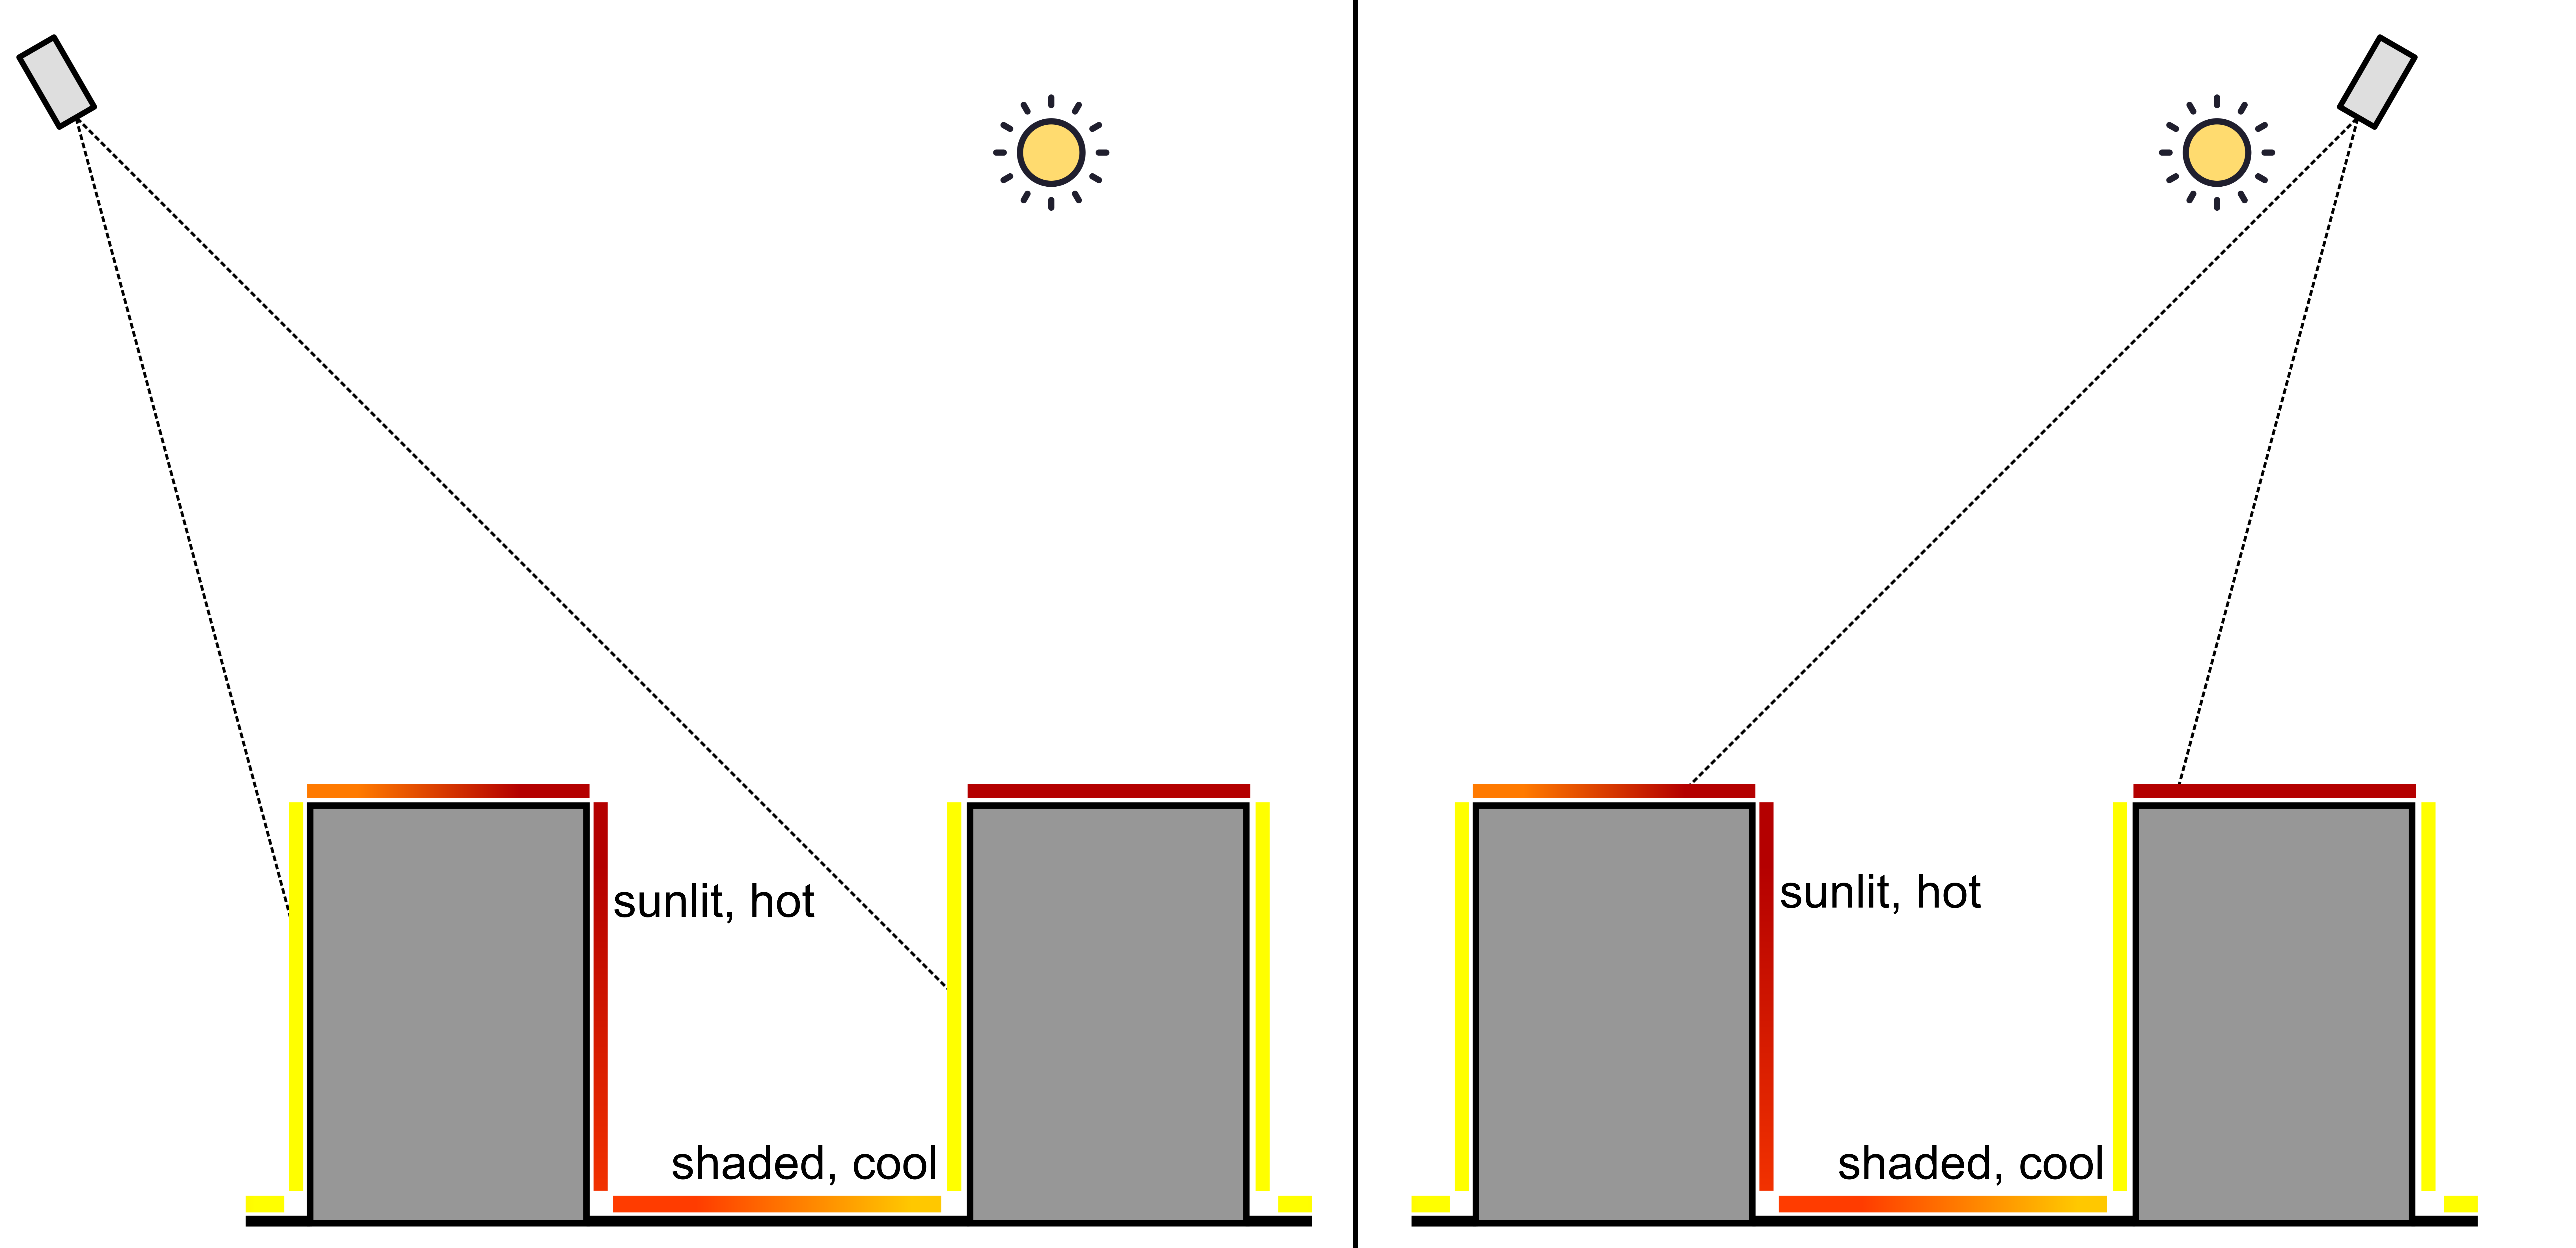
\includegraphics[width=15cm,
	height=7in,
	keepaspectratio]{anisot}
	\caption{A narrow-FOV sensor viewing an idealized urban surface from two angles. Left: viewing the surface approximately perpendicular to the sun's angle. Right: viewing the surface approximately parallel to the sun's angle. The two viewing angles yield different remote sensed T\textsubscript{surf} by sampling different arrangements of sunlit and shaded features. Both will deviate from an area weighted "complete" urban T\textsubscript{surf}.}
	\label{anisot}
\end{figure}

Geometric undersampling by narrow-FOV remote sensors results in remote sensed urban T\textsubscript{surf} changing based on a sensor's viewing direction and the assemblage facets included within the sensor FOV. A sensor viewing the surface perpendicular (parallel) to the sun's angle will tend to underestimate (overestimate) the "true" complete urban surface temperature - often calculated as an area weighted average of wall, rooftop, and road T\textsubscript{surf} - by differentially biasing sunlit or shaded facets. Similarly, a sensor in the nadir will tend to overestimate daytime urban T\textsubscript{surf} and underestimate nighttime T\textsubscript{surf}, from a bias towards differentially hot (cool) rooftop facets by day (night) and a neglect of wall facets which are differentially cooler (warmer) by day (night). As the effect of geometric biases is highly dependent on surface-sensor-sun geometry and requires significant instrumentation for quantification, its influence in the remote sensed sUHI record is presently unknown.

Temporal biases in thermal remote sensing of urban areas occur across multiple time scales including: 

\noindent---\textit{Contamination by turbulence forced, high frequency fluctuations in urban T\textsubscript{surf}}. 

Using time-sequential thermography \citet{Christen2012} found that many common urban fabric types (e.g. rooftops, walls, roads, and vegetation) display large micro-scale (second to minute) fluctuations in T\textsubscript{surf}. The magnitude of which is inversely related to surface thermal admittance and is, as of writing, poorly understood. Most thermal remote sensors provide instantaneous, rather than temporally averaged, T\textsubscript{surf} and thus are subject to contamination by high-frequency fluctuations. These biases are difficult to estimate in urban environments, where a large variety of fabric materials can produce significant directional contrasts in thermal admittance - and thus spatial variations in the magnitude of microscale fluctuations depending on the facet material types viewed by the sensor. 

\noindent---\textit{Discontinuity in satellite overpass cycles.}

Satellite overpass cycles are discontinuous. Assessment of land T\textsubscript{surf} either sacrifices spatial resolution for a daily repeat cycle - as is the case with MODIS  - or sacrifices temporal resolution for a higher spatial resolution - ASTER or Landsat. Geostationary satellites do not currently have sufficient spatial resolution to resolve coherent urban pixels.

\noindent---\textit{Clear-sky bias.}

Clouds absorb TIR – thus satellite TIR remote sensing of the surface requires clear sky conditions. Although the urban effect on T\textsubscript{surf} is most evident under "satellite friendly" clear sky conditions (manifesting as large sUHI magnitudes), a clear sky bias likely entails overestimation of "all-sky" sUHI and further adds to discontinuities in the remote sensed urban T\textsubscript{surf} record.

As is the case with geometric biases, the magnitude of these temporal biases in remote sensed urban T\textsubscript{surf} is difficult to quantify without long-term ground truthing campaigns or significant interpolation. Thus, the true temporal and geometric nature of urban effect of T\textsubscript{surf} is presently unknown.
 
\section{Research questions and objectives}

Prompted by these shortcomings in the remote sensed urban T\textsubscript{surf} record, and in an effort to better understand the temporal and geometric aspects of sUHI, this thesis introduces a method to provide hemispherical, temporally continuous urban T\textsubscript{surf} for sUHI analysis to address the following questions:

\begin{enumerate}
	\item What is the nature of urban surface temperature when viewed from a hemispherical downward-facing radiometer? And how does it relate to urban temperatures derived from other methods for urban surface temperature retrieval?
	\item What is the diurnal and seasonal nature of the surface urban heat island effect?
\end{enumerate}

\noindent In an attempt to answer these questions, I did the following:

\begin{itemize}
	\item Developed and evaluated a method to retrieve atmospherically correction hemispherical radiometric urban surface temperatures from time-continuous measurements of upwelling longwave radiation.
	\item Compared urban surface temperatures and surface urban heat island magnitudes retrieved using the method to common remote sensed representations of the urban surface.
	\item Derived an eight month climatology of hemispherical urban surface temperatures to observe seasonal and diurnal patterns of the surface urban heat island effect.
\end{itemize}

The following two chapters address questions one and two respectively. Chapter \ref{paper1} details and evaluates a method to retrieve atmospherically corrected, hemispherical urban T\textsubscript{surf} from time-continuous measurements of upwelling longwave radiation. Chapter \ref{paper2} explores the temporal and geometric nature of sUHI through an eight month climatological analysis of hemispherical sUHI and compares sUHI magnitudes from several representations of the urban surface.


\cleardoublepage 
\phantomsection  
\renewcommand*{\bibname}{References}
\addcontentsline{toc}{section}{\textbf{References}}

\putbib
\end{bibunit}

\chapter{A method to correct upwelling longwave radiation to estimate hemispherical urban surface temperature}

\section{Introduction}
Thermal infrared (TIR) remote sensing of land surface temperature (T\textsubscript{surf}) has emerged as a primary research focus in climatology, as researchers seek to better describe spatiotemporal patterns of T\textsubscript{surf} globally and better understand how anthropogenic modification of earth's surface influences land T\textsubscript{surf} with links to the climate at-large. Over the last two decades, use of thermal remote sensing of surface climates has expanded significantly --- both in terms of the volume and breadth of remote sensed study and its explicative importance in climatology as a discipline. Thermal remote sensing of earth's surface has applications over a wide range of disciplines: from informing micro-, urban-, and global-scale climate models, to aiding decision making and mitigation praxis with respect to climate change and the \gls{uhi}. 

Within urban climatology, a combination of satellite, aerial, and ground-based thermal remote sensors have been integral in elucidating the spatial \cite{Roth1989}, temporal \cite{Peng2012}, and geometric \cite{Voogt1997} effects of the built environment on land T\textsubscript{surf}; in evaluating and partitioning urban surface energy balances \cite{BastiaanssenW.G.M.1998, Yamaguchi2005} and; in characterizations of the relationship between surface and \gls{blayer} air temperatures (T\textsubscript{air}) \cite{Stoll1992}. These advances have been aided by substantial improvements in sensor ground, spectral, and radiometric resolutions, and by the proliferation of both large-scale public satellite remote sensing campaigns and low-cost aerial and near-ground thermography. However, in spite of it's widespread usage, several questions concerning the use and validity of urban remote thermal remote sensing, first posed in Roth et al. 1989 \cite{Roth1989}, have yet to be sufficiently answered, viz,

\begin{enumerate}
	\item What is the nature of the surface 'seen' by a thermal remote sensor?
	\item How does T\textsubscript{surf} observed by a remote sensor relate to the 'true' temperature governing the surface-atmosphere interface?
\end{enumerate}

\noindent In this paper, we seek to examine question two by introducing and evaluating a method for atmospheric and emissivity correction of near-ground hemispherical TIR --- measured via \gls{pyrg} --- for hemispherical radiometric temperature (T\textsubscript{hem}) retrieval. These measures are common to most urban energy balance assessments and thus constitute a hitherto untapped method for urban T\textsubscript{surf} analysis. A companion paper responds to question one through an analysis of a climatology of T\textsubscript{hem} and derived surface UHI (sUHI), to quantify geometric and temporal biases across multiple methods for remote sensing of urban T\textsubscript{surf}.

\section{Atmospheric effects on TIR}

Although most thermal remote sensors operate within one of the \gls{atmwind}[s] --- where atmospheric effects are greatly reduced --- virtually any remote sensed TIR signal is subject to radiative effects from the layer of atmosphere between the surface and the sensor. Over much of the thermal infrared \gls{waveband} the atmosphere emits radiation and absorbs a fraction of radiation emitted by the surface. Thus, a remote sensed TIR signal almost certainly not equal to the ground emitted signal. For an isothermal, homogeneous surface-atmosphere system, at-sensor spectral radiance at height ($z$) can be described by a function deviating from a Planck curve at T\textsubscript{surf} based on the spectral transmittance of the intervening atmosphere, with the magnitude of that deviation governed by the difference between Planck curves at T\textsubscript{surf} and the ambient T\textsubscript{air}. As shown for two path geometries in \ref{spectairtsurf} for an atmosphere with water vapor content of  12 g/m\textsuperscript{3} and aerosol and trace gas profiles from the mid-latitude summer standard atmosphere, an at-sensor spectral radiance signal deviates significantly from the surface emitted spectral radiance curve. A less transmissive atmosphere increases the potential for deviation in the at-sensor signal from the ground emitted signal, while the difference between T\textsubscript{air} and T\textsubscript{surf} determines the resulting magnitude of atmospheric influence on the spectral TIR signal.

\begin{figure}[!ht]
	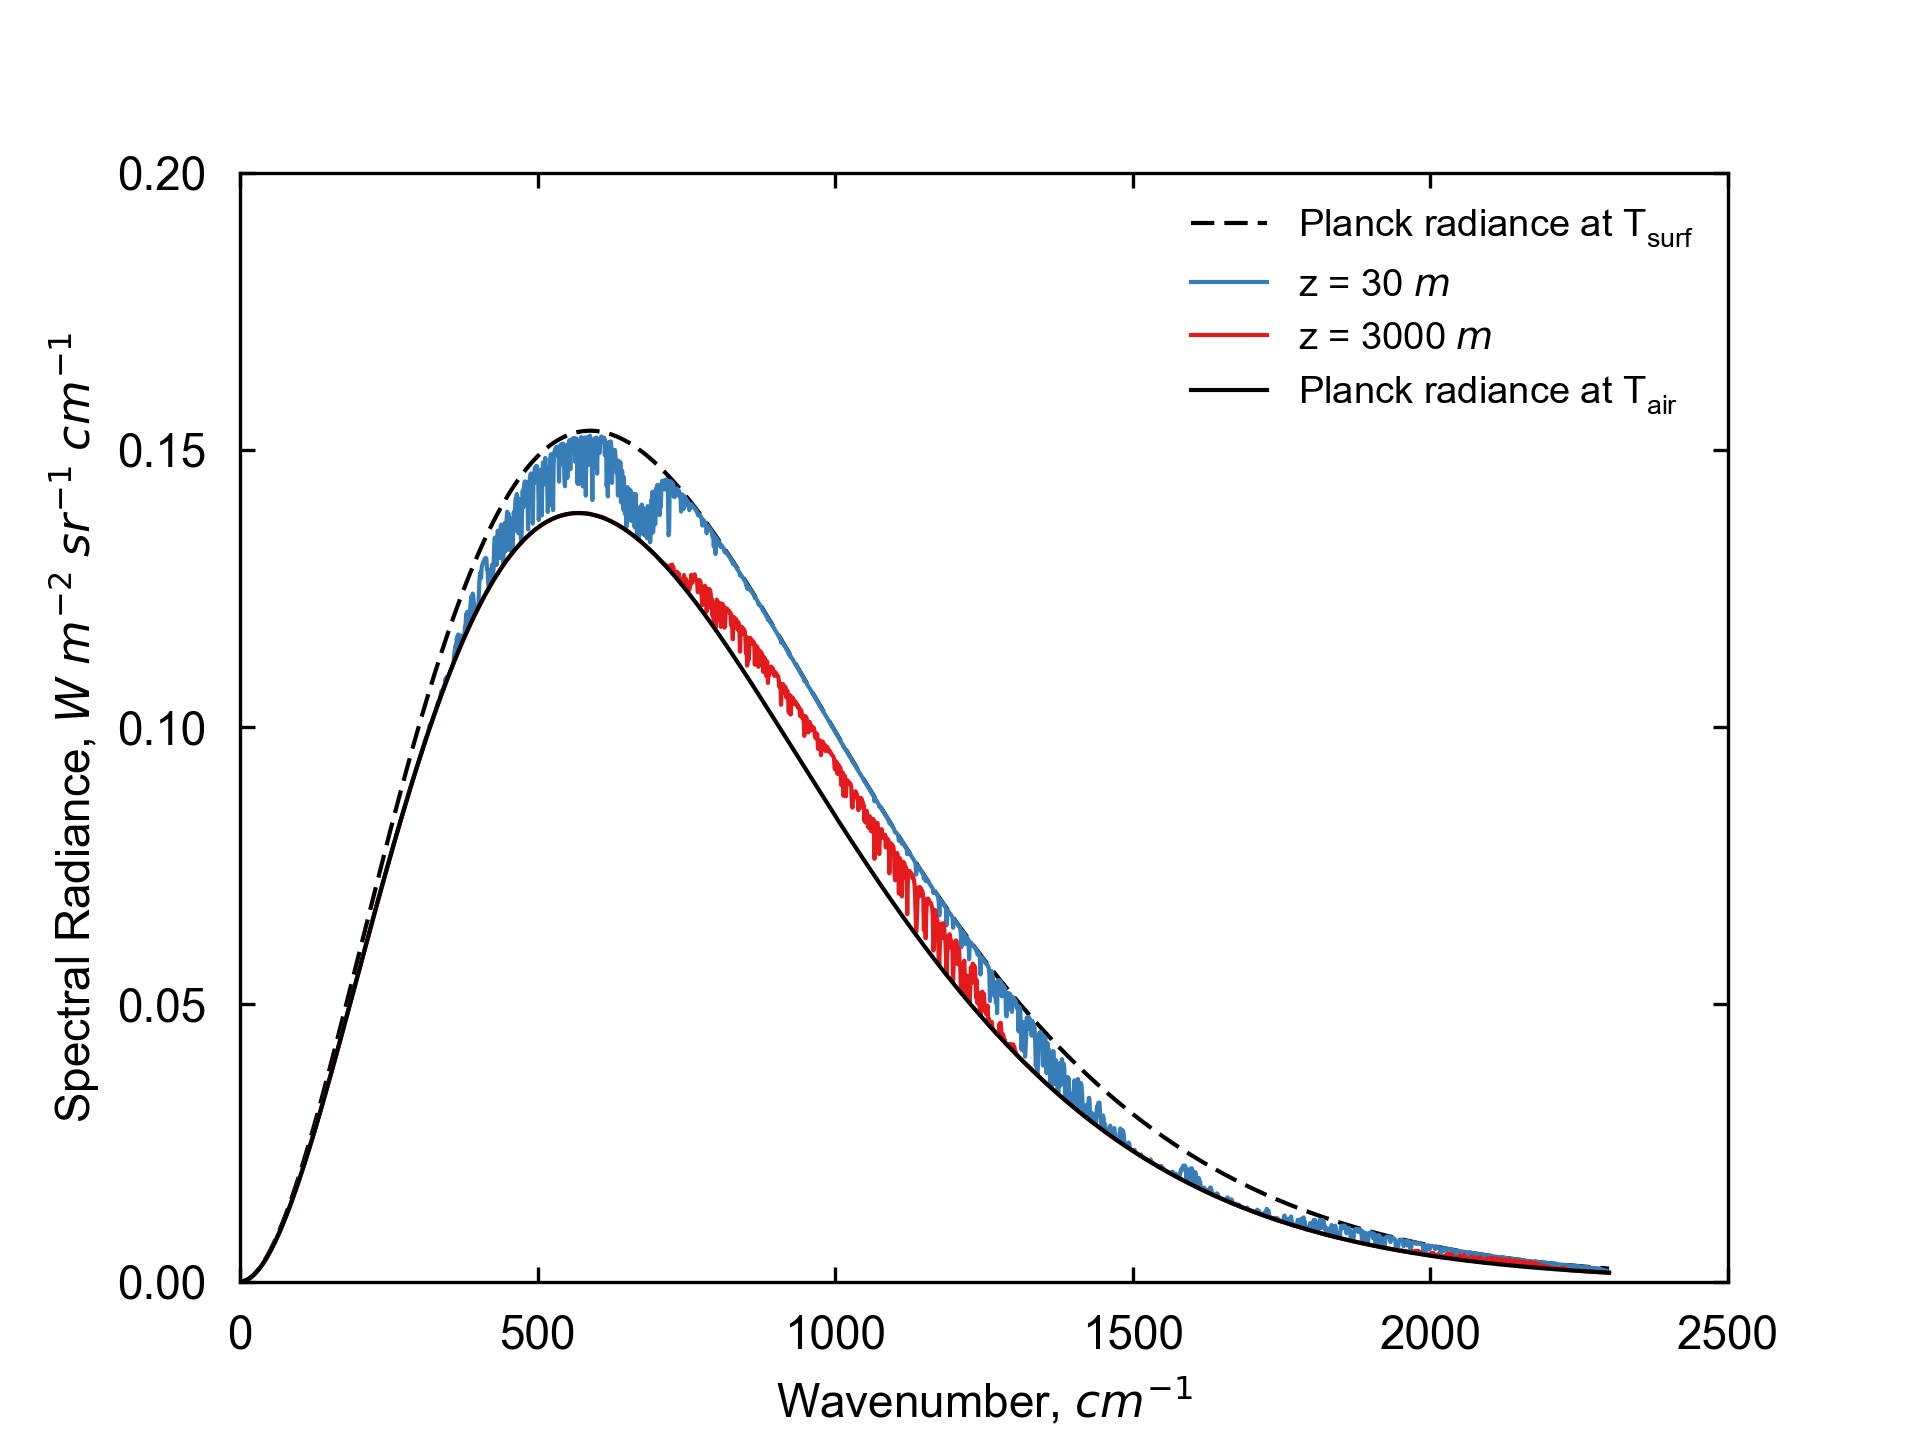
\includegraphics[width=\textwidth]{spectairtsurf}
	\caption{At-sensor spectral directional radiances computed in MODTRAN 4.1 \cite{Berk1987} for short (30m) and long (3000m) path lengths (z) with Planck curves indicating spectral radiances at T\textsubscript{air} = 305 K and T\textsubscript{surf} = 295 K.}
	\label{spectairtsurf}
\end{figure}

Atmospheric effects can lead to differences between the 'true' radiometric T\textsubscript{surf} and the remote sensed T\textsubscript{surf} of over 10 k for satellite platforms \cite{Cooper1989} and over 6 K for near-ground sensors \cite{Meier2011}. Moreover, because atmospheric and emissivity effects are a function of non-uniform and spatiotemporally variant surface and atmospheric properties, their associated errors change depending on instrument type, surface-sensor geometry, study location, and ambient conditions. As intersite and time-sequential analysis is a significant goal of most thermal remote sensed studies (urban or otherwise) these effects cannot be ignored.

Spectral transmission of longwave radiation through a given layer of atmosphere is dependent on total column absorber content (the principal broadband TIR absorbers are H\textsubscript{2}0, C0\textsubscript{2}, and to a lesser extent 0\textsubscript{3}, N\textsubscript{2}0, CO, CH\textsubscript{4}, and 0\textsubscript{2} \cite{Miskolczi1993}). Holding vertical absorber content constant, variation in band-by-band TIR transmittance with path length is greatest at urban scales (approximately 1 to 50 meters), where transparent spectral bands can quickly become opaque with small changes in path length or absorber content - illustrated in figure \ref{spectransheight}. Thus, transmittance of TIR near the surface is highly dependent on surface-sensor geometry, instrument spectral response, and atmospheric absorber content. Indeed, accurate assessment of atmospheric influence on TIR may be most complex when measured near the surface.

\begin{figure}[H]
	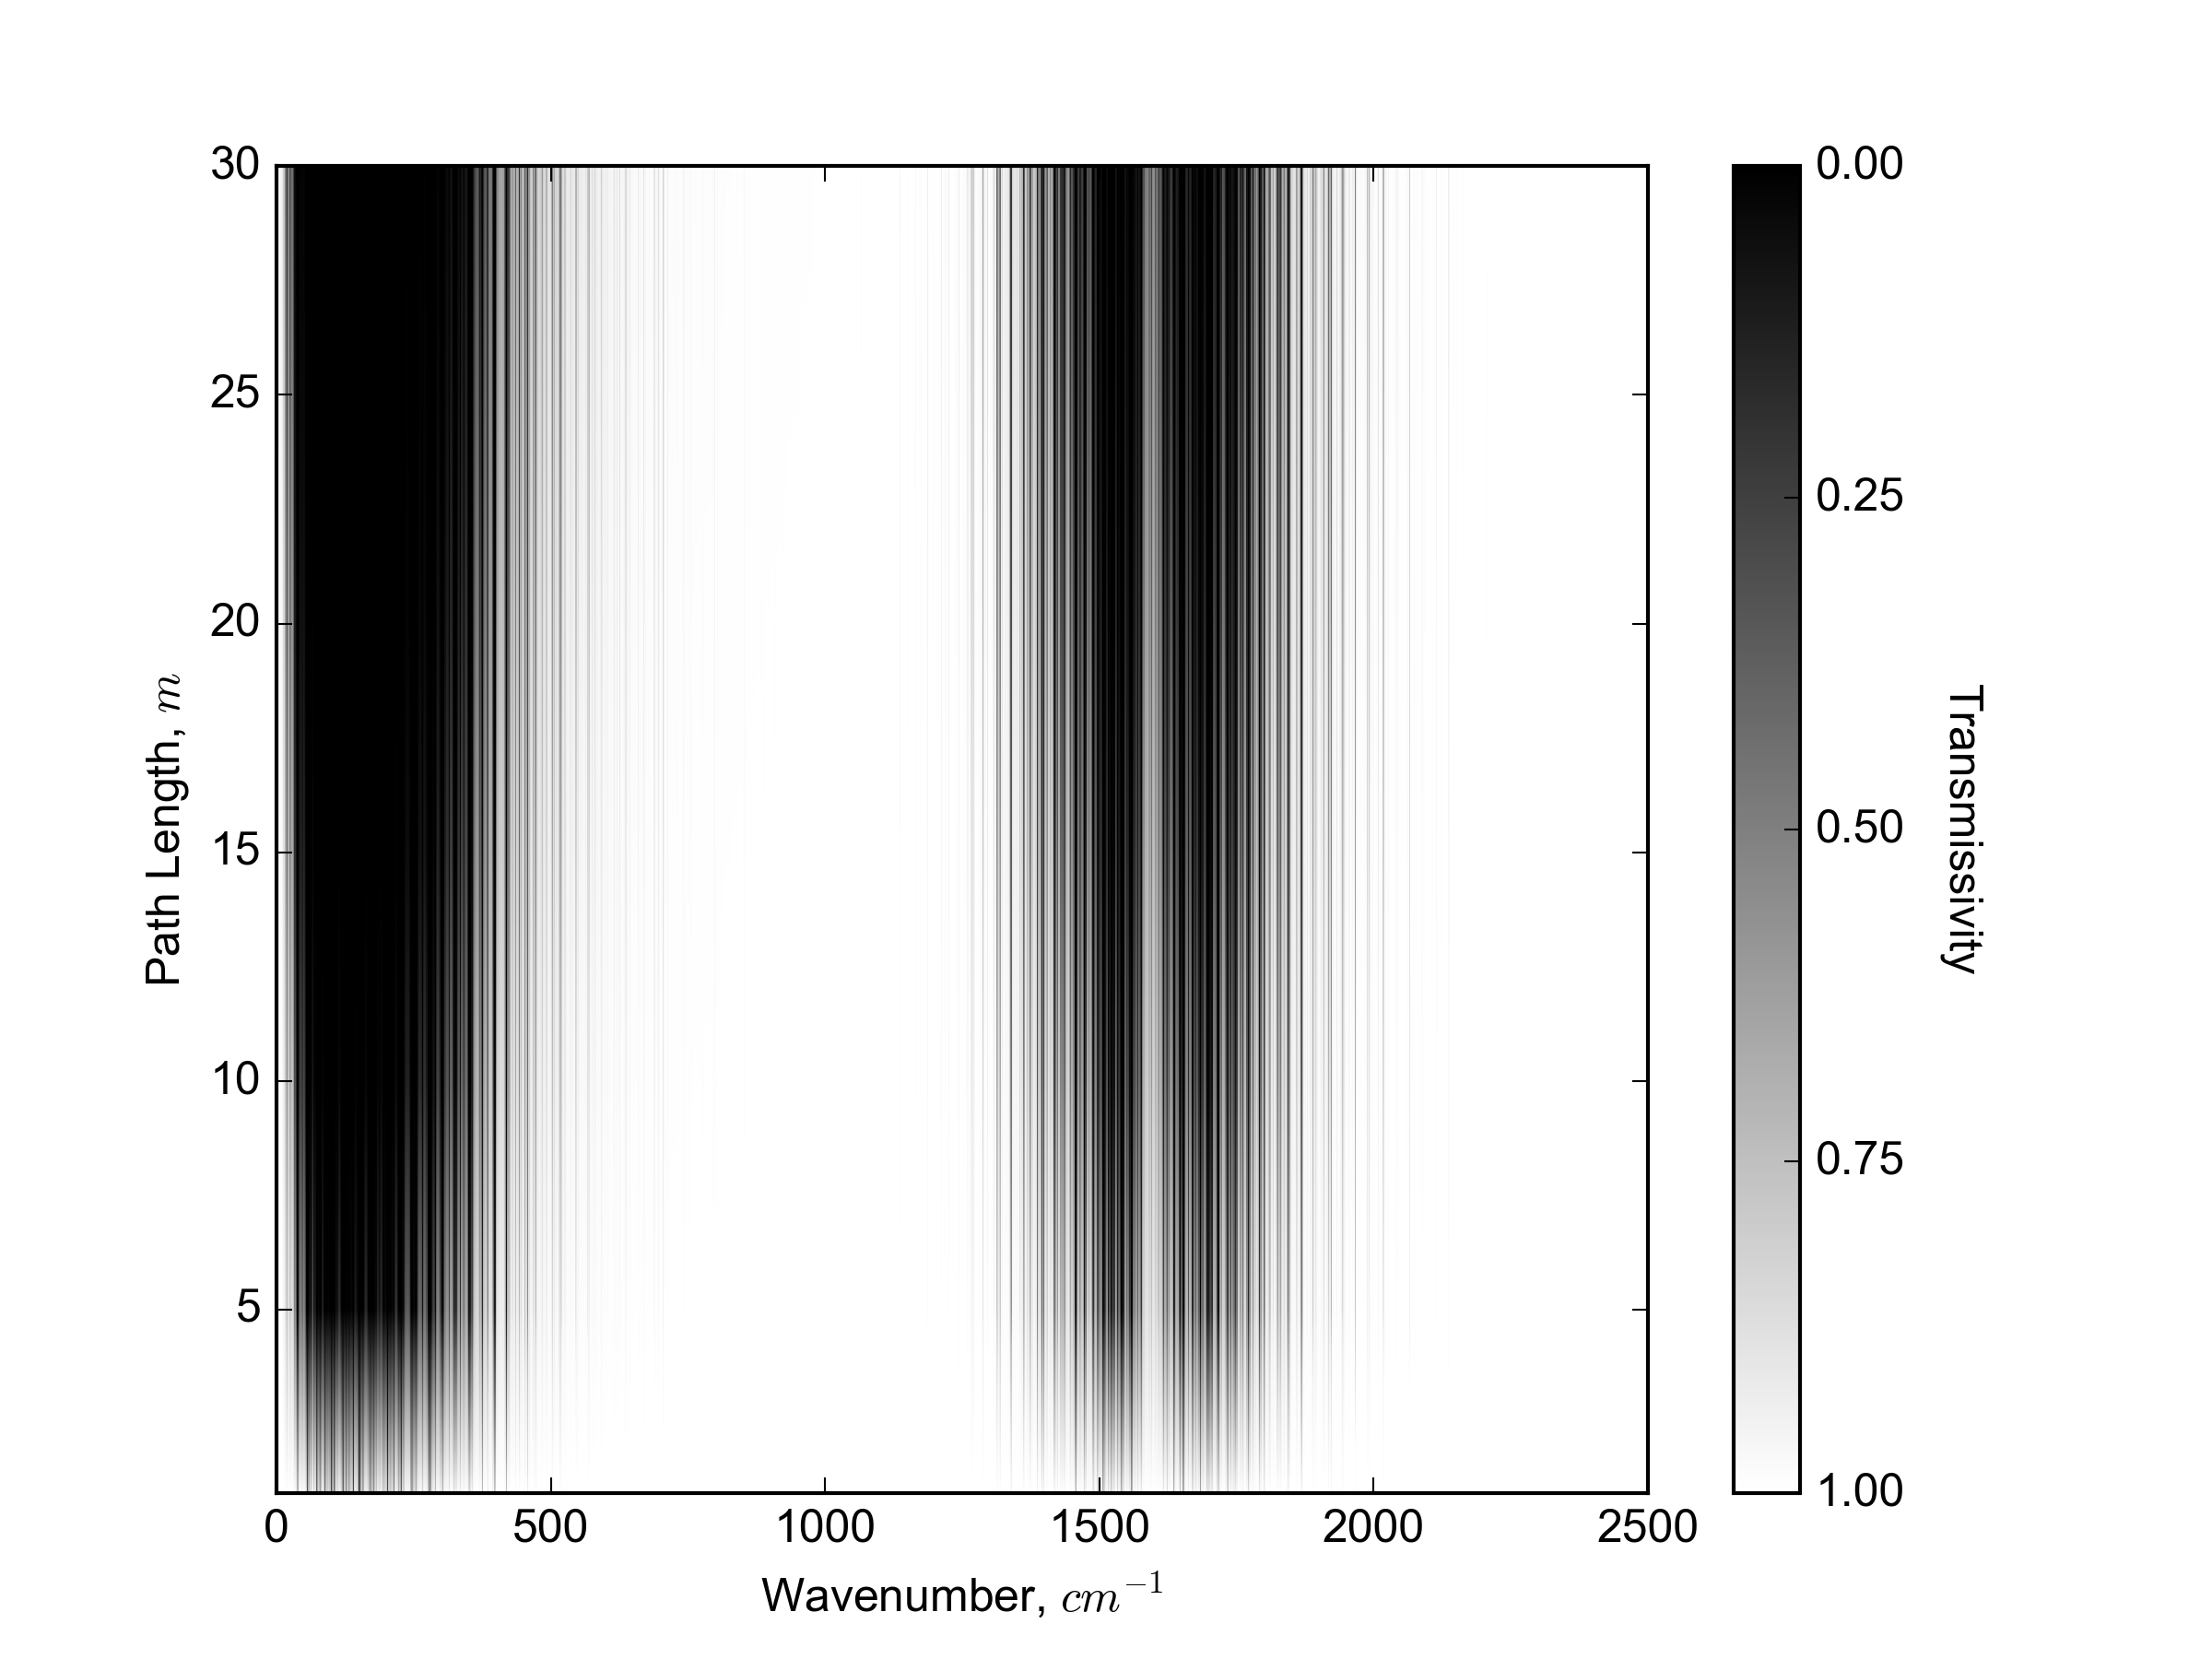
\includegraphics[width=\textwidth]{spectransheight}
	\caption{Spectral transmission of water vapor as a function of height. Black and grey shading indicate opaque (0\% transmittance) and transparent (100\% transmittance) bands respectively. Redo this figure with wavelength and colorbar no totle and the tick marks in back on the outside?}
	\label{spectransheight}
\end{figure}

Radiation passing through a layer of atmosphere from an emitting surface can be described in a number of ways. \textit{Spectral directional radiance} $ R (\lambda)$, at height $ z $ and from a direction defined by zenith angle \(\theta\), and azimuth angle \(\phi\) is commonly written as

\begin{equation}
R^\uparrow_z (\lambda, \theta, \phi) = \tau_\lambda \epsilon R^\uparrow_0(\lambda) + (1-\epsilon) R^\downarrow_{sky} (\lambda) + (1-\tau_\lambda) R^\uparrow_{atm}(\lambda)
\end{equation}

\noindent where \(\epsilon\) is surface emissivity, \(\tau\)\textsubscript{\( \lambda \)} is spectral "slab" transmittance through the layer between the emitting surface $( z  = 0) $ and $ z $. The same spectral TIR signal, as measured by a narrow-FOV sensor mounted at height $ z $, passes through an instrument shield (or dome) with spectral transmittance \(\tau_d\), and is integrated over the sensor waveband (bounded by \(\lambda_1\) and \(\lambda_2\)) to yield a \textit{directional radiance} $L'$ as 'seen' by the sensor

\begin{equation}
L'_z (\theta, \phi) = \int_{\lambda_1}^{\lambda_2} \tau_d(\lambda) R^\uparrow_z(\lambda) ~ d\lambda
\end{equation}

\noindent which, integrated over the hemisphere with respect to zenith \(\theta\) angle and azimuth \(\phi\) angle, yields an \textit{irradiance} $ L $ at height $ z $,

\begin{equation}
L_z = \int_{0}^{2\pi} \int_{0}^{\pi/2} L_z'(\theta, \phi) ~ \cos\theta \sin\theta ~ d\theta d\phi
\end{equation}

\subsection{Relating TIR and surface temperature}

TIR received by a remote sensor can be related to the emitting body's temperature in a number of ways --- each producing different conceptions of T\textsubscript{surf} from different instrument and sensor types. As such, the term "surface temperature" with respect to a remote sensed TIR is vague and can refer to several definitions of "surface" and "temperature" Thus, proper terminology must be attached to land T\textsubscript{surf} inferred from TIR. Definitions and nomenclature conventions for multiple methods for T\textsubscript{surf} retrieval are discussed at length in Norman \& Becker, (1995)\cite{Norman1995}.

Directional radiance $ L'_z $ detected from a narrow-FOV sensor operating over waveband (\(\lambda_1\) --- \(\lambda_2\)) and viewing the surface from some orientation described by \(\theta\), \(\phi\) can be used to infer a \textit{directional brightness temperature} T'\textsubscript{bright}(\(\theta\), \(\phi\)) via an inversion of the Planck function multiplied by normalized sensor response integrated over the sensor waveband,

\begin{equation}
L'_z(T'_{bright} (\theta, \phi)) = \bigints_{\lambda_1}^{\lambda_2} \cfrac{f(\lambda) C_1}{\pi \lambda^5 \left( \exp\left(\cfrac{C_2}{\lambda T'_{bright} (\theta, \phi)}\right)\right)}
\end{equation}

\noindent where C\textsubscript{1} = $ 3.7404 \cdot 10^8 $ $ W\mu^4 m^{-2} $, C\textsubscript{2} = $ 14387 \mu K $, and relative sensor response $ r(\lambda) $ normalized via,

\begin{equation}
1 ~ =  \int_{\lambda_1}^{\lambda_2} r(\lambda) ~ d\lambda
\end{equation}

Similarly irradiance $L_z$ received by a broadband hemispherical sensor (such as a pyrgeometer), can be used to infer a \textit{hemispherical brightness temperature} T\textsubscript{bright} through an inversion of the Stefan-Boltzmann law,

\begin{equation}
\label{stefb1}
L_z = \overline{r} (\sigma T_{bright}^4)
\end{equation}

\noindent where $ \sigma $ is the Stefan-Boltzmann constant and $ \overline{r} $ is Planck weighted average broadband sensor response computed as,

\begin{equation}
\overline{r} = \cfrac{\int R(\lambda) ~ r(\lambda)}{\int R(\lambda)}
\end{equation}

\noindent with $ R(\lambda) $ computed from a Planck function at an approximated $T_{bright}$. 

In addition, a simple approximation of $T_{bright}$ can be inferred from directional radiance using equation \ref{stefb1} by replacing $ L_z $ with $L'_z$ multiplied by a constant. This method is commonly used to infer T\textsubscript{bright} from infrared thermometers (IRT) operating over the atmospheric window (where atmospheric correction magnitudes are small and T\textsubscript{bright} is a reasonably accurate approximation of T\textsubscript{surf}). However, constants must be calibrated for the range of expected T\textsubscript{surf} as the relationship between $ L_z $ and $L'_z$  is not perfectly linear.

Inversions of uncorrected directional radiances or irradiances using the Planck function or the Stefan-Boltzmann law yield a temperature equal to that of a blackbody emitting the same amount of radiation as detected by the sensor. Since $ L_z $ is unlikely to be equal to $ L_0 $, T\textsubscript{bright, 0} and T\textsubscript{bright, z} often show significant variation based on sensor characteristics, ambient conditions, and surface-sensor geometry. Hence, remote sensed T\textsubscript{bright} is generally considered only a rough approximation representation of kinetic or thermodynamic T\textsubscript{surf}. 

To retrieve a more accurate estimation of the 'true' T\textsubscript{surf}, the same inversions can be applied to TIR measurements after correction for atmospheric and surface emissivity effects (e.g. transformations of the TIR signal to represent that at $ z = 0 $ if the surface was emitting as a perfect blackbody) to yield a direction radiometric surface temperature T\textsubscript{rad} for atmospheric and emissivity corrected directional radiances, a hemispherical radiometric surface temperature T\textsubscript{hem} for atmospheric and emissivity corrected irradiances. $ T\textsubscript{rad} (\theta, \phi) $ and T\textsubscript{hem} provide a better approximation of the ‘true’ T\textsubscript{surf} by representing the temperature at which the surface is radiating integrated over the sensor FOV.


\subsection{Atmospheric correction of near-ground TIR} \label{Atmospheric correction of near-ground TIR}

A large number of correction routines have been developed to remove atmospheric and emissivity effects from aerial and satellite TIR signals and derive accurate T\textsubscript{rad}. Methods range from simple mono- \cite{Qin2001} and split-window \cite{Wan1996} routines for single- and multi-channel remote sensors to schemes that integrate a radiative transfer code to isolate the surface emitted signal from interfering signals. Boundary conditions are standard across most correction methods: generally requiring vertical profiles of T\textsubscript{air}, humidity, pressure, and aerosol content to remove atmospheric effects, and assessments of surface radiative properties to correct for emissivity effects. However, correction methods are often instrument (or at least platform) specific and difficult to generalize across sensor and platform types. Few methods exist for correction of ground based remote sensed TIR --- none of which are robust enough to correct irradiances upwelling from rough terrain measured via wide-\gls{fov} (FOV) radiometers. In part, this is due to the fact that until recently, errors inherent in radiometer measurements were large relative to atmospheric effects. However, a new breed of more accurate radiometers and thermal imagers should prompt a critical reevaluation of this assumption.

Atmospheric correction of near-ground remote sensed TIR is subject to a unique set of challenges compared to traditional satellite and aerial platforms. Near-ground and wide-FOV remote sensors have complex, multiple line-of-sight (LOS) geometry - illustrated in figure 2.1 for a downward facing hemispherical radiometer. Surface-sensor geometry varies significantly over the sensor FOV, even when measured close (less than 5m) above the surface. The addition of 3-dimensional surface geometry further amplifies this effect, as some paths may intersect with raised vertical, sloped, and horizontal features. This creates the potential for non-uniform atmospheric effects over the sensor FOV and necessitates a multi-LOS correction to retrieve accurate T\textsubscript{rad}. In effect, with near-ground wide-FOV sensors, surface geometry is non-trivial and must be represented in atmospheric correction routines. In contrast, over a scene retrieved via satellite, spatial viability in surface geometry and LOS angle have a negligible effect on path length. Atmospheric correction routines for satellite retrieved TIR, therefore, assume uniform or single-LOS geometry because the TIR signal passes through a relatively constant volume of atmosphere over the projected sensor FOV, regardless of surface geometry. This greatly increases the complexity of correction routines for near-ground wide-FOV radiometry. 

\begin{figure}[!ht]
	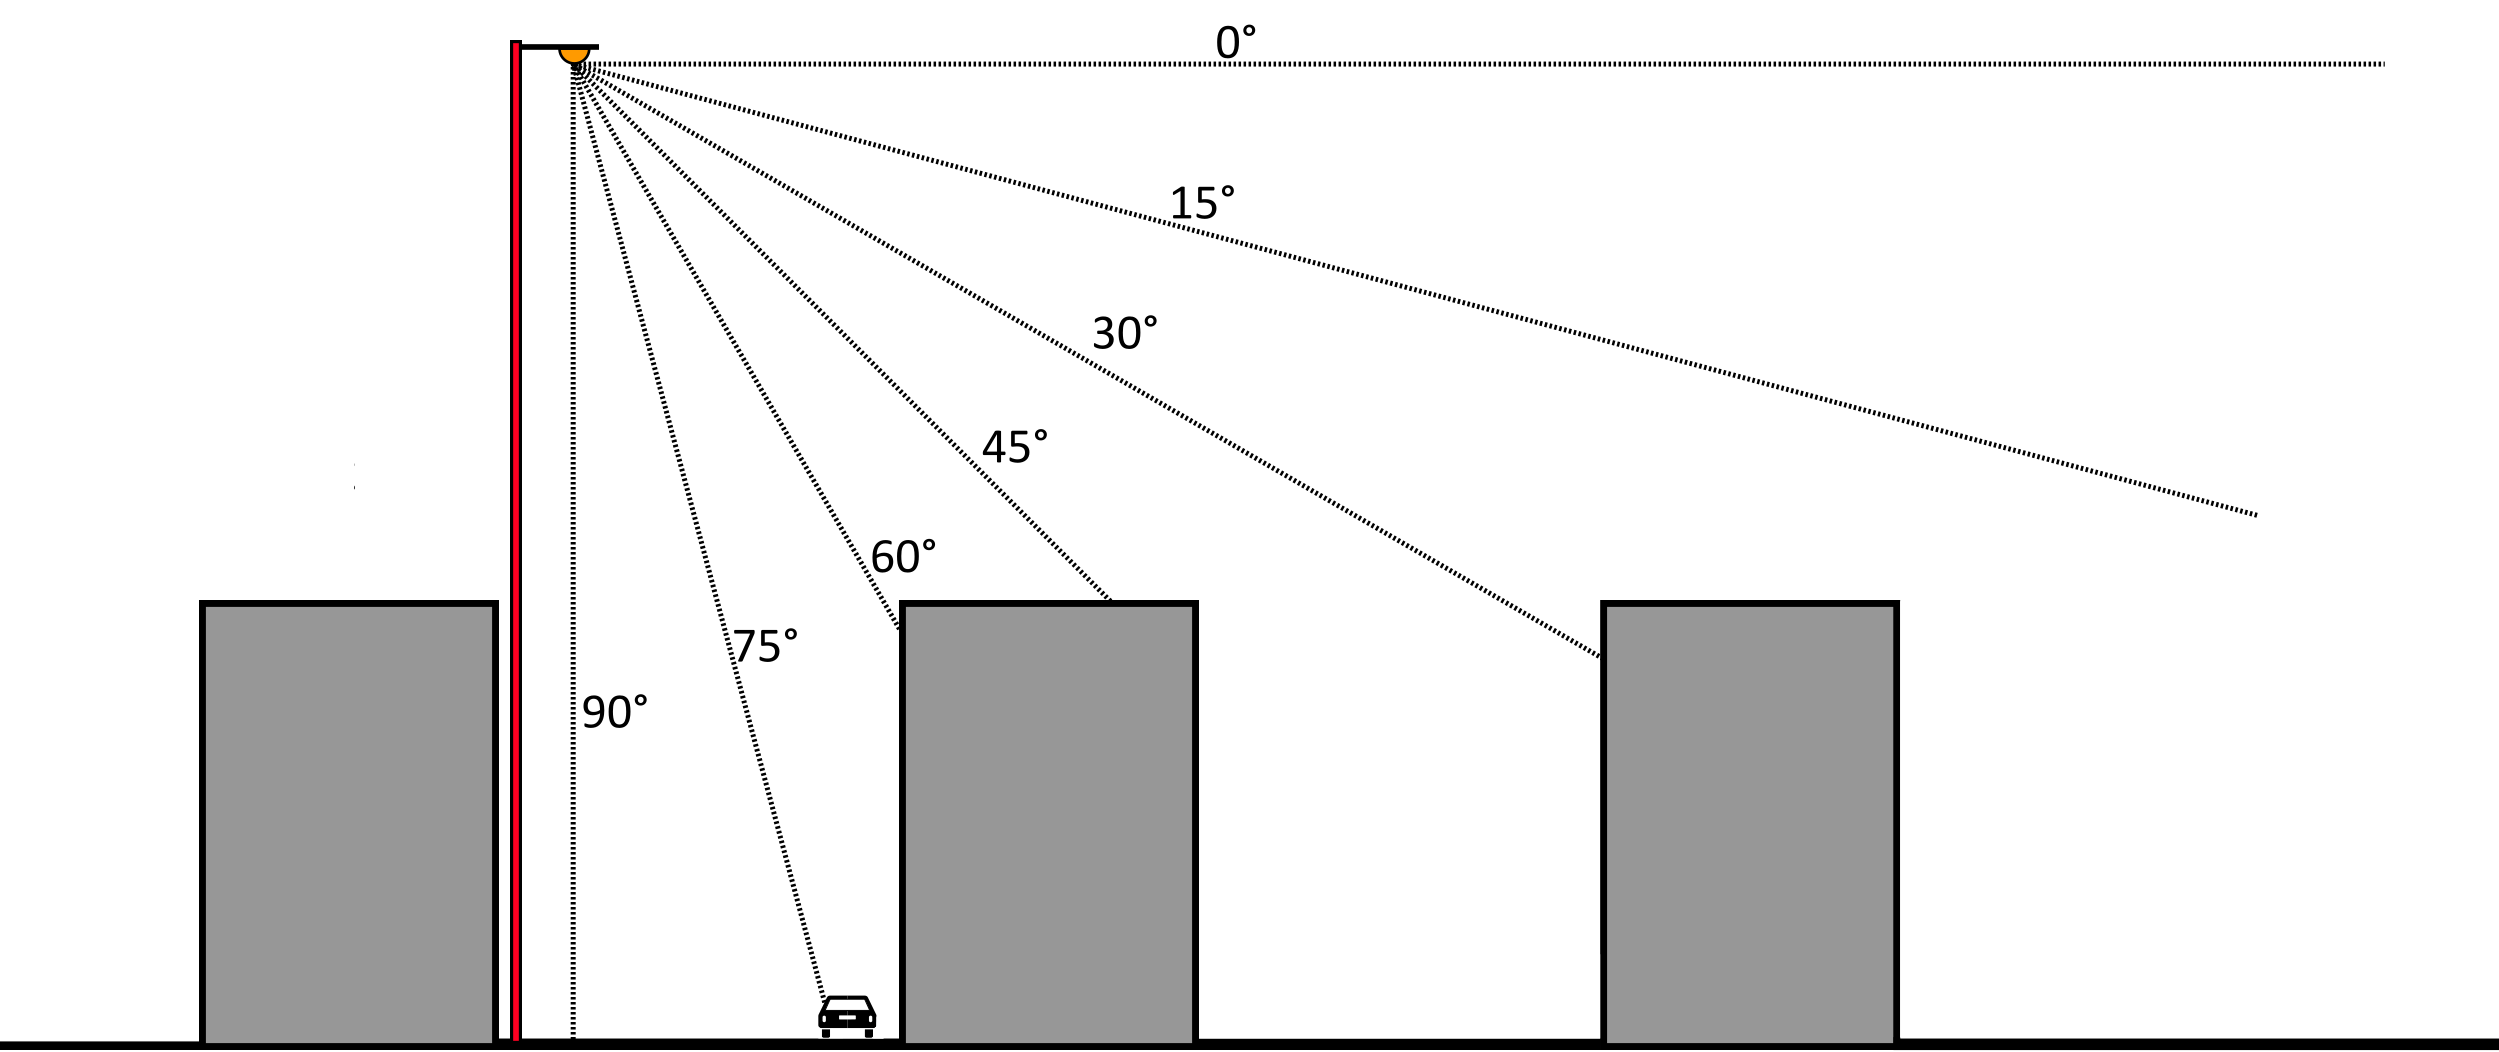
\includegraphics[width=\textwidth]{lineofsight}
	\label{lineofsight}
	\caption{Variable path geometry inherent with wide-FOV near-ground sensor visualized over an idealized 2-dimensional urban area.}
\end{figure}

Several multi-LOS atmospheric correction routines have been developed for near-ground TIR: Meier et al., 2011 describes a correction method for oblique angled urban thermography \cite{Meier2011}. Path lengths were calculated for each pixel over the FOV of a tower-mounted thermal imager angled obliquely toward the urban surface. A correction factor was then computed and applied using a radiative transfer code initialized using isothermal, isohumal atmospheric profiles for each time step. Applied over a time-series of images, the result is a continuous atmospherically corrected series of thermal images with each pixel representing a different T\textsubscript{rad}. However, the method uses visual-band images and a GIS database to represent urban geometry for each pixel's LOS - a technique not possible with a pyrgeometer, which returns a single integrated irradiance at each time-step. Moreover, the target instrument operates over a narrow waveband, reducing the magnitude and variance in atmospheric transmission over the sensor response curve. Thus, the method is not directly generalizable to correction TIR as measured via pyrgeometer.  Kotani \& Sugita, 2009 describes a method for correction of wide-FOV (pyrgeometer) TIR Irradiances \cite{Kotani2009a} over planar terrain. However, these methods are limited to narrow-FOV thermal imagers and sensors over planar surfaces respectively. A method which combines Meier et al., 2009's representation of complex surface geometry and Kotani \& Sugita, 2009's broadband hemispherical integration is needed for atmospheric correction of urban TIR measured from a downward facing pyrgeometer. A method to correct hemispherical broadband TIR as measured from a downward facing pyrgeometer needs to combine the two for accurate T\textsubscript{hem} retrieval over rough terrain. 

\section{A "rolling lookup table" method for hemispherical atmospheric correction}

%alt title:method to retrieve atmospherically corrected hemispherical surface temperatures from near ground TIR

The "rolling lookup-table" method described in this study uses a sensor view model in conjunction with a radiative transfer code to model hemispherical irradiances upwelling from a simplified isothermal 3-dimensional representation of the target study area. In summary, the method (depicted in figure \ref{flow}) uses vertical profiles of measured T\textsubscript{air} and humidity to model at-sensor spectral radiances at 5$^{\circ}$ increments over the sensor FOV for a predefined range of possible T\textsubscript{hem} at each time-step. Spectral directional radiances are convolved by a dome transmittance curve, integrated over the sensor waveband, and weighted for their respective angular view factor. Weighted directional radiances are then integrated over the hemisphere and aggregated into a lookup table (LUT) of modeled irradiance---T\textsubscript{hem} pairings for each timestep, unique to the vertical profile of measured T\textsubscript{air} and humidity. Finally, for each time-step, measured irradiances are matched with the closest modeled irradiances in the associated LUT to return an atmospherically corrected hemispherical surface temperature (T\textsubscript{hem}). This process is repeated at 30 minute intervals to yield a continuous climatology of urban T\textsubscript{hem} for surface urban heat island (sUHI) analysis. The following sections introduce the study area and describe the sensor view modeling, radiative transfer, and post-processing steps of the method.



\begin{figure}[!ht]
	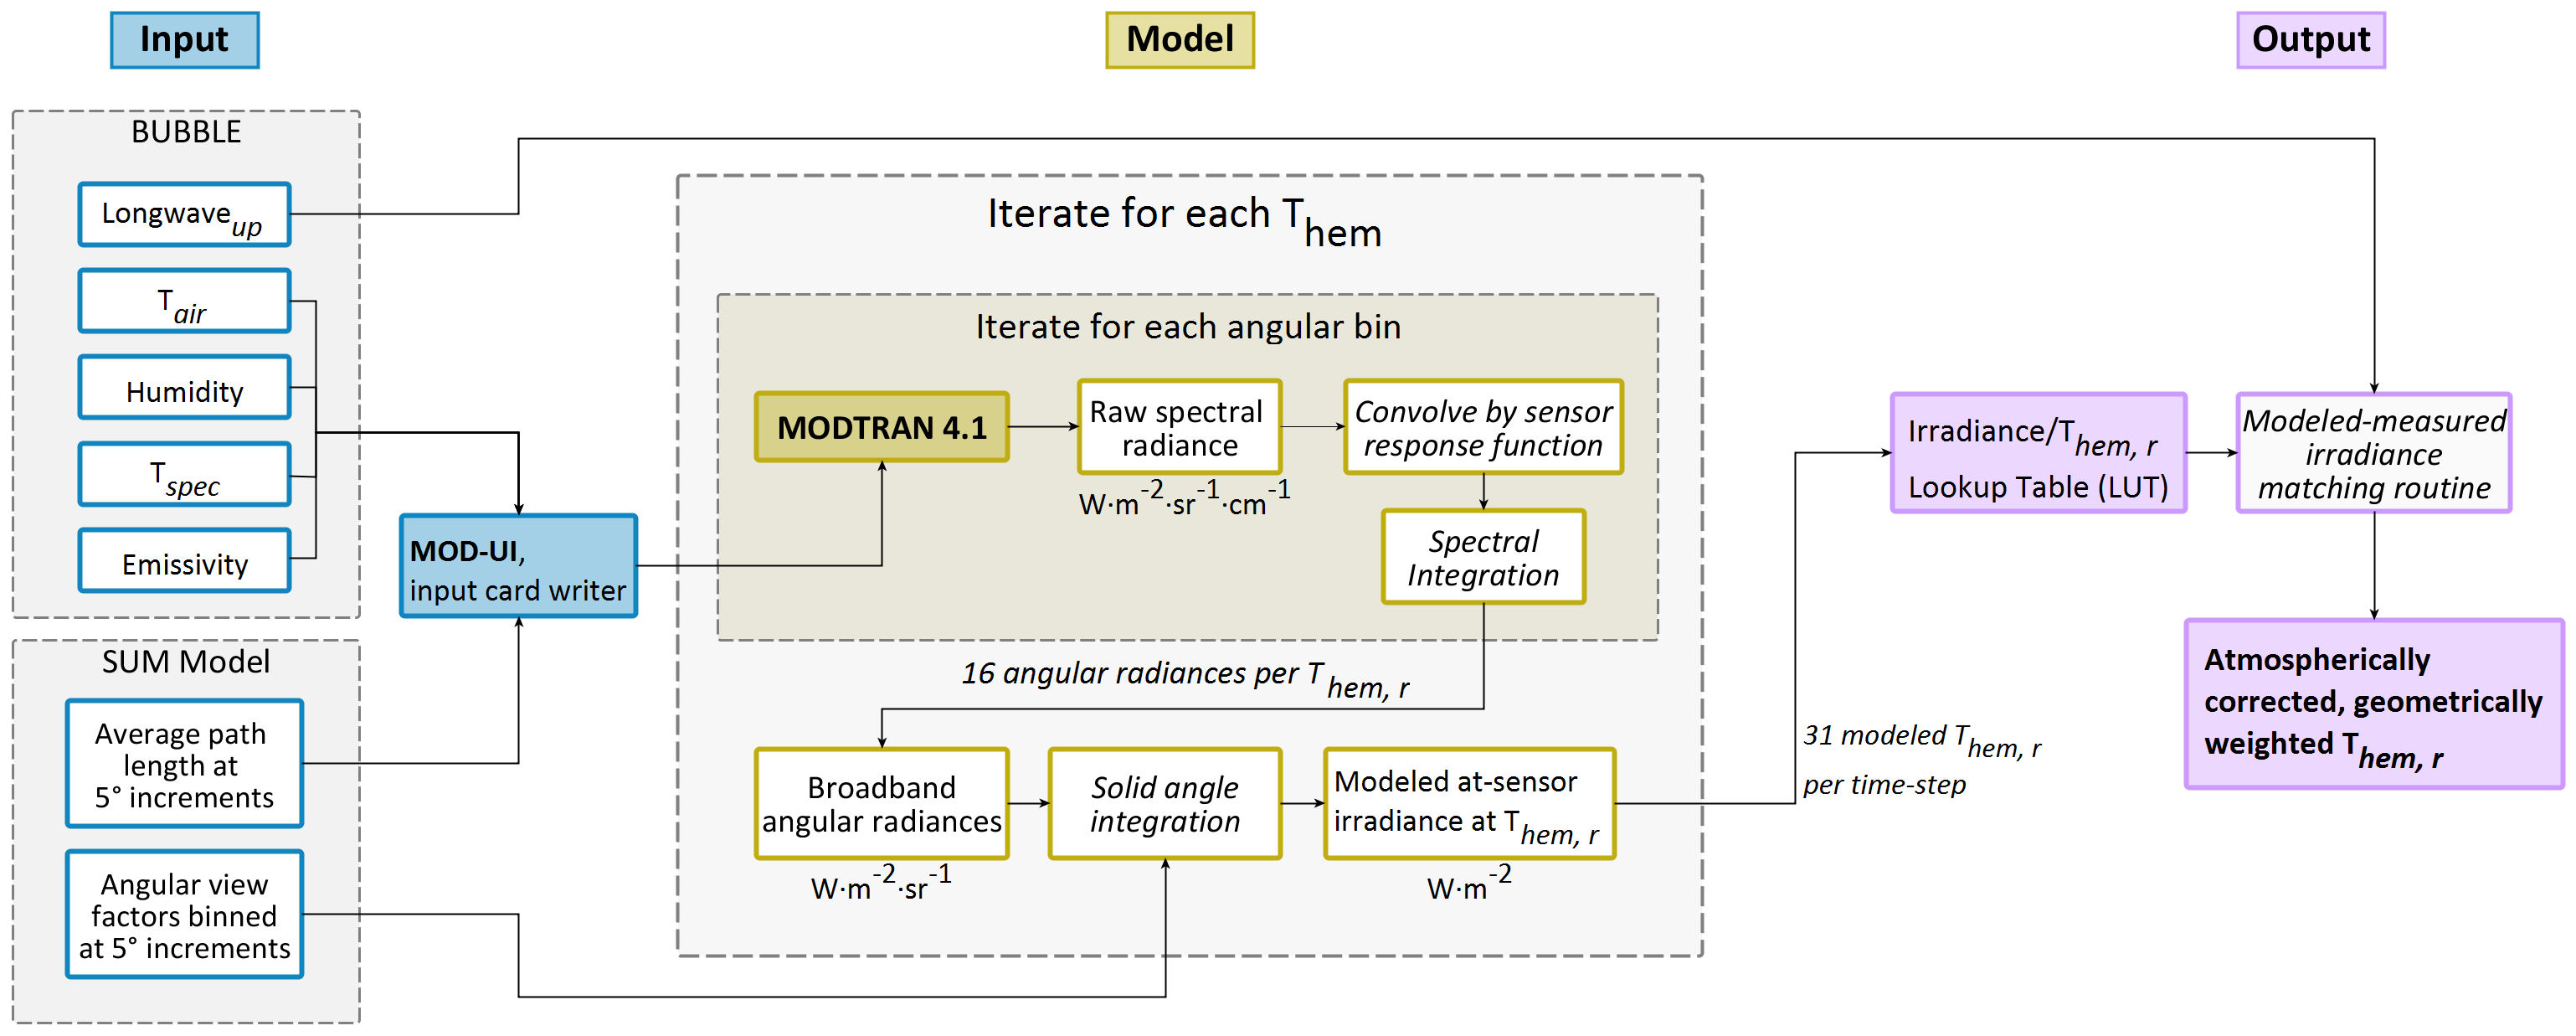
\includegraphics[width=\textwidth]{flow}
	\label{flow}
	\caption{A workflow schematic depicting the input, model, and output-processing steps of a "rolling lookup table method" for hemispherical radiometric surface temperature retrial.}
\end{figure}

\subsection{Study area}

As discussed in Section \ref{Atmospheric correction of near-ground TIR}, atmospheric correction of longwave irradiances measured from downward-facing, near-ground, wide-FOV sensors must account for surface geometry - particularly when mounted to view complex surface geometry. Hence, routines to retrieve atmospherically corrected urban T\textsubscript{hem} from upwelling longwave irradiances are inherently site specific. However, it is important to note that although correction magnitudes described in this paper are not generalizable, the correction method described in this paper can readily be adapted to different study sites, pyrgeometer types, and unique surface geometries.

With methodological generalizability in mind, a "rolling lookup table" atmospheric correction method was developed to retrieve radiometric T\textsubscript{hem} for a climatology of upwelling longwave irradiances measured from above the Sperrstrasse urban street canyon in Basel, Switzerland. The site, instrumented as a part of the Basel Urban Boundary Layer Experiment (BUBBLE) \cite{Rotach2005}, has an approximately northeast-southwest orientation and site morphology representative of local climate zone (LCZ) 2\footnote{Site surroundings can be described by the following morphological parameters: mean building height: 14.6m, plan aspect ratio: 0.54, complete aspect ratio: 1.92, local canyon aspect ratio: 1.0, and average shortwave albedo: 0.11 \cite{Rotach2005}.} \cite{Stewart2012}. LCZ classification was based on an assessment of surface characteristics in a 250m circular area extending from the Sperrstrasse tower using a 1m raster digital building model (DBM). Thus, the morphological parameters identified in \cite{Rotach2005} are representative of the vast majority of the pyrgeometer footprint. However, it should be noted that vegetation was not included in the DBM, and thus is not represented in morphological assessment or the sensor view model. 

For the nine month period between November 2001 and July 2002, a triangular lattice tower was installed skewed towards the southeast facing wall near the center of the Sperrstrasse canyon to observe a full suite of meteorological, radiation, and flux parameters. Profiles of T\textsubscript{air} and humidity were measured from seven heights extending from 2.5m to 31.5m above the canyon floor (with the highest observation level at approximately 2.17 times mean building height). Upwelling and downwelling short/longwave fluxes were measured at the lowest and highest tower heights, with an additional downward facing pyrgeometer mounted at roof level in the center of the canyon. In addition, during a summertime intense operation period (IOP) an array of narrow-FOV IRTs was installed to view individual facet surface temperatures (T\textsubscript{facet}) of approximately the same urban patch viewed by the pyrgeometer. 

The BUBBLE Sperrstrasse site was chosen for two primary reasons: 1. The study site provided a long-term climatology of radiation and meteorological variables for a representative mid-latitude city over a diverse range of synoptic conditions. This allowed for examination of urban T\textsubscript{surf}, atmospheric correction magnitudes, and sUHI magnitudes over a wide range of mid-latitude conditions. 2. T\textsubscript{facet} measured during the summertime IOP allowed for direct climatological comparison of T\textsubscript{hem} to wall (T\textsubscript{wall}), roof (T\textsubscript{roof}), and road (T\textsubscript{road}) surface temperatures of both the northwest- and southeast-facing sides of the canyon. In addition, several hypothetical sensor views of the canyon were simulated by weighting to represent different geometric representations of the canyon, including a nadir/plan view, an oblique south-facing, and an oblique north-fac from narrow-FOV sensors and a complete, 3-dimensional view of the canyon. This facilitated comparison of T\textsubscript{hem} against different instrument types and platforms to identify and quantify biases in each method.  In each representation, different weightings were applied to T\textsubscript{wall}, T\textsubscript{roof}, and T\textsubscript{road} on both sides of the canyon to represent different sensor orientations and sampling regimes. Weightings for each representation are described in table \ref{weightings}. 
\begin{table}[!ht]
	\centering
	\caption{Weightings to produce T'\textsubscript{rad} for different geometric representations of the Basel street canyon.}
	\label{weightings}
	\begin{tabular*}{\textwidth}{l@{\extracolsep{\fill}} p{1cm}p{1cm}p{1cm}p{1cm}p{1.6cm}}
		\toprule 
		& Road & Northwest & Southeast & Northwest & Southeast \\ 
		&  & Roof & Roof & Wall & Wall \\ 	\midrule

		Complete & 0.33 & 0.16 & 0.16 & 0.16 & 0.16 \\ 

		Nadir & 0.46 & 0.27 & 0.27 & 0.00 & 0.00 \\ 

		Oblique (south-facing) & 0.20 & 0.25 & 0.25 & 0.00 & 0.30 \\ 

		Oblique (north-facing) & 0.20 & 0.25 & 0.25 & 0.30 & 0.00 \\ 
		\bottomrule
	\end{tabular*} 
\end{table}

\subsection{Modeling path lengths of 3-dimensional terrain}

The sheer number of unique path length geometries inherent with wide-FOV radiometry of rough terrain makes full 3-dimensional radiative transfer simulation difficult and computationally intensive --- particularly when correcting a climatology of T\textsubscript{hem}. In this method, to improve model efficiency, radiances are calculated for azimuthally averaged path lengths that represent average surface terrain for each solid angle "slice" of the sensor FOV. Thus, hemispherical radiative transfer is reduced to a 2-dimensional problem (shown in panel (b) of figure \ref{23radtran}). This greatly reduces the computational time required to model each irradiance-T\textsubscript{hem} pairing, as angular radiances can be computed as a function of zenith angle alone and subsequently weighted and integrated 3-dimensionally over the hemisphere. 

To calculate surface-sensor geometries, the Surface-Sensor-Sun Urban Model (SUM) \cite{Soux2004} is initialized with a simplified, orthogonal 3-dimensional DBM representing the street canyons and courtyards immediately surrounding the sensor. SUM uses a four-dimensional array to represent surface morphology   with three spatial dimensions ($x$, $y$, and $z$), with $z$ representing height above the $x$, $y$ plane. SUM also includes an additional fourth dimension, where properties describing each cell are stored (in this case, distance from the point to the sensor). After specifying sensor FOV and position relative to the DBM, the model determines which patches have an unobstructed line of sight to the sensor and calculates the distance from "seen" patches to the sensor. Path lengths are binned at 5$^{\circ}$ increments of zenith angle and averaged to return an azimuthally-independent mean path length for each bin. In addition, while simulating path length geometries, SUM calculates view factors for each solid angle "slice", which are later used to weight 2-dimensional angular radiances in the hemispherical integration post-processing steps.

\begin{figure}[!ht]
	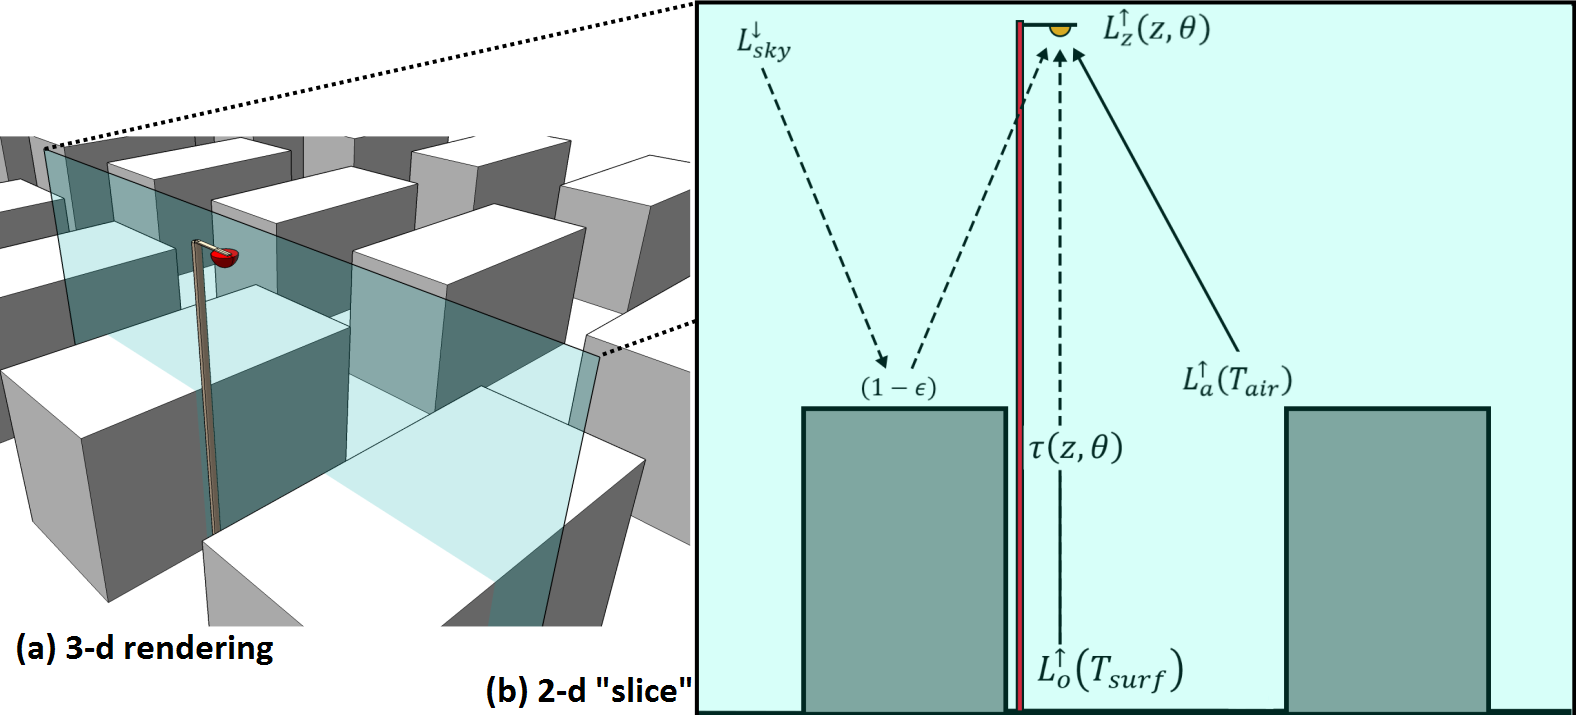
\includegraphics[width=\textwidth]{23radtran}
	\label{23radtran}
	\caption{A typical 2-dimensional (b) radiative transfer schematic adapted for an idealized 3-dimensional urban area (a). In 3-dimensions, path length for a given zenith angle can change significantly with azimuth angle. Dotted lines indicate the potential for absorption by the intervening atmospheric layer}
\end{figure}

\subsection{Modeling hemispherical irradiances}
With path length geometries calculated in SUM, irradiances are modeled time-sequentially using the MODerate resolution atmospheric TRANsmission 4.1 radiative transfer code (MODTRAN) \cite{Berk1987}. At each time-step, a range of potential T\textsubscript{hem} is selected using T\textsubscript{bright} subtracted by some constant (6 K during nighttime runs and 4 K for daytime runs). In MODTRAN, at-sensor spectral radiances for each path length are modeled over a waveband of 0---2500cm\textsuperscript{-1} at 0.5 K intervals over the range of potential T\textsubscript{hem}. Atmospheric profiles are constructed from 30-minute averages of T\textsubscript{air} and humidity with aerosol and above-sensor conditions are informed by the mid-latitude summer standard atmosphere when daytime maximum T\textsubscript{air} is greater than 10 $^{\circ}$C (the mid-latitude winter profile is substituted on days with T\textsubscript{air, max} of less than 10 $^{\circ}$C). 
Spectral radiances are convolved by a dome transmittance.




\section{Evaluation of the method using profiles of upwelling longwave radiation over a homogenous planar surface}

MODTRAN has been shown to effectively model near-ground radiative transfer at urban-scale path lengths in 2-dimensions. However, the method detailed in this paper includes significant post-processing to ‘collate’ point-to-point radiances into 3-dimensional hemispherical irradiances. In addition, the method accounts for site-specific surface geometry, which has a significant influence on boundary-layer transmittance of broadband longwave radiation. Thus, prior to deriving a climatology of radiometric urban Them, the method was evaluated over a simple surface with known surface characteristics. Thus, divergences are solely the result of differential atmospheric effects with increasing height above ground, which should be accounted for by the model. It is assumed that each pyrgeometer in this validation views a patch with approximately the same temperature. 

Profiles of upwelling longwave radiation, downwelling shortwave, air temperature, and humidity at 2m, 10m, and 30m were obtained from the Payerne station, located 50 miles southwest of Basel, Switzerland in a cultivated field. To evaluate the method, we used a modified version of the workflow described in XXXX. Brightness temperature calculated from the lowest upwelling longwave measurement was used to model irradiances at 10m and 30m at each time-step. Downwelling shortwave radiation was used to categorize test days based on cloud cover. The daytime air temperature profile was modified to replicate typical lapse rates in the Sperrstrasse canyon. Unlike, Kotani \& Sugita (2009), an isothermal atmospheric profile was not sufficient to accurately model upwelling longwave divergences (nor fluxes) of planar terrain. Although thermal stratification is likely to be relatively small by day in an urban canyon \cite{Nakamura1988} --- where strong microscale contrasts in Tsurf foster canyon mixing and neutral stability --- the large daytime Tsurf-T\textsubscript{air}  differential and the path-length/transmittance gradient can create large positive divergences (5 – 15 Wm\textsuperscript{-2},CHECK THIS). As such, we suggest using a full canyon T\textsubscript{air} /humidity profile to 

Modeled upwelling longwave at 10m and 30m and divergences are compared to their measured counterparts in figure a. Both fluxes and divergence show strong correlations, thus we conclude: 1. Irradiances measured at 2m are free from significant atmospheric influence – as an uncorrected irradiance provided an accurate Tsurf for modeling of 10m and 30m Irradiances As such, brightness Them and radiometric Them are approximately equal when z < 2m. Although, it should be noted that a 2m sensor is not representative of canyon geometry and should not be used to derive urban Them. 2. The method is sensitive enough to model divergences in a large layer above a flat surface. Urban divergences are likely to be smaller with less frequent and less severe stable stratifications. Thus, we can safely make the assumption that the method is effective over complex terrain – provided path length geometries are accurately replicated in SUM.




\chapter{A climatology of urban surface heat islands derived from hemispherical radiometric surface temperatures}

\section{Introduction}

The temperature of the surface is integral in understanding, predicting, and modeling boundary-layer air temperature patterns, surface energy balances, and, in urban areas, has important implications for human thermal comfort and building energy usage. Urban modification of surface geometry and thermal, radiative, moisture, and aerodynamic properties results in differential surface heating and cooling patterns and strong microscale spatiotemporal variations in urban surface temperature (T\textsubscript{surf}). Integrated up to larger scales, urban areas tend to store and generate more heat relative to non-built surroundings which manifests in elevated T\textsubscript{surf} and T\textsubscript{air} --- a phenomenon termed the urban heat island effect (UHI). To foster a more complete understanding of the effect of urban areas climates across scales, accurate, spatiotemporally continuous and geometrically representative characterization of T\textsubscript{surf} in cities has long been a goal in urban climatology. The proliferation of satellite and aerial thermal infrared (TIR) remote sensing has enabled spatially-extensive characterizations of surface climates at ever improving spatial and spectral resolutions. Such campaigns have elucidated urban T\textsubscript{surf} and surface urban heat island (sUHI) patterns globally at large spatial scales. However, technological improvements in TIR remote sensing have yet to address a three potential sources of error when applied in urban areas: 

\begin{enumerate}
	\item Geometric undersampling of 3-dimensional terrain
	\item Temporal discontinuity in overpass cycles and sensor sampling regimes
	\item Clear-sky bias
\end{enumerate}

\noindent These biases present a potentially significant source of error by failing to capture micro-scale temporal and geometric variations in urban T\textsubscript{surf} and sUHI. 

Inter-site comparison is the crux of UHI analysis, thus it is imperative that urban T\textsubscript{surf} measurements are representative of coherent urban patches and free from confounding influences (i.e. atmospheric and emissivity effects). Meta-analysis of air temperature (T\textsubscript{air}) UHI literature shows that these goals are rarely satisfied \cite{Stewart2011}. Given the relative difficulty in retrieving accurate, representative urban T\textsubscript{surf}, similar conclusions are likely for sUHI analysis. In spite of this fact, and the short period over which large-scale, generalizable methods for measuring urban T\textsubscript{surf} have been available, study of sUHI via TIR remote sensing has expanded significantly in the last twenty years \cite{Peng2012,Voogt2003}. Using the method described in \ref{paper1} we derive an 8-month climatology of hemispherical radiometric urban T\textsubscript{surf} (T\textsubscript{hem, r}) from time continuous near-ground upwelling TIR as measured from an inverted pyrgeometer. The method was developed to address and overcome biases inherent in traditional methods for urban T\textsubscript{surf} retrieval by providing temporally continuous, geometrically representative\footnote{A hemispherical view is not perfectly geometrically representative of urban surface geometry. This is best illustrated by visualizing an urban area from the perspective of a downward facing ‘fish-eye’ camera. Geometric sampling biases are a result of lens distortions and the sensor cosine response. However, by sampling the surface 3-dimensionally, T\textsubscript{hem, r} is more representative of urban geometry than conventional 2-dimensional views of the surface. The geometric representivity of urban T\textsubscript{hem, r} is discussed in section \ref{Methodological limitations and considerations}.} urban T\textsubscript{surf} under all-sky conditions for sUHI analysis. These measurements are often made as a part of the net radiation determination for urban energy balance studies.

\subsection{Bias in thermal remote sensing}
Geometric biases in remote sensing of the urban surface are a result of its 3-dimensional, convoluted structure. Compared to flat terrain, complex urban surface geometry modifies receipt of incoming solar radiation and traps a portion of reflected solar and outgoing terrestrial radiation. The resulting microscale spatiotemporal contrasts in urban T\textsubscript{surf} create a directional dependence in observed urban T\textsubscript{surf} when measured from conventional narrow-field-of-view (FOV) TIR remote sensing platforms. Thus, remote sensed urban T\textsubscript{surf} varies based on sensor FOV, viewing angle and direction, and sun-surface geometry - this directional dependence of urban surface temperature is termed "effective thermal anisotropy" \cite{Voogt1998a}. Traditional satellite or airborne remote sensing platforms, by viewing the surface in the nadir, sample only a fraction of the complete urban surface and fail to capture this effect - leading to spatiotemporally variant directional biases of up to 10 \si{\kelvin} in observed urban T\textsubscript{surf} \cite{Voogt1995}. In general, geometric undersampling by a remote sensor in the nadir manifests as an overestimation of daytime T\textsubscript{surf} and an underestimation of nighttime T\textsubscript{surf} \cite{Adderley2015}. However, the magnitude and diurnal and seasonal behaviors of this bias are dependent on sensor viewing geometry and unique site characteristics (canyon height-to-width ratio, canyon orientation and materials, vegetation coverage, etc.). Thus, parameterization schemes to account for urban effective anisotropy are difficult to generalize across urban sites, sensor types, and sensor-surface geometries.

In addition to undersampling the urban surface, most thermal remote sensing platforms yield an instantaneous ‘snap-shot’ and cannot characterize time-continuous T\textsubscript{surf} patterns without sacrificing ground resolution. Temporal discontinuities in thermal remote sensing result in myriad of potential sources of bias over a wide range of time scales. Aerial and satellite thermal remote sensing require clear sky conditions (clouds are opaque with respect to thermal infrared radiation). Hence, long term satellite characterizations of sUHI are biased towards conditions that maximize urban-rural contrasts in T\textsubscript{surf}. This results in an overestimation of “all-sky” sUHI. At diurnal scales, satellite overpass cycles rarely coincide with sUHI maximums and are not standard across cities or platforms. Thus, analysis of sUHI patterns and magnitudes across cities and instrument platforms is difficult. At smaller time scales still, time-continuous analysis of urban T\textsubscript{surf} shows significant microscale (second to minute) fluctuations in temperature \cite{Christen2012}. Most thermal remote sensors provide instantaneous T\textsubscript{surf} (rather than temporally averaged) and are potentially contaminated by high-frequency microscale fluctuations in urban T\textsubscript{surf}. This is particularly salient in urban environments, where a large variety of fabric materials can produce significant directional contrasts in thermal admittance - and thus spatial variations in the magnitude of microscale fluctuations depending on the facet material types viewed by the sensor. The effect of this phenomenon on thermal remote sensing has not been extensively studied, however, the magnitude of microscale fluctuations in T\textsubscript{surf} is significant relative to a typical sUHI signal and thus constitutes a potentially large source of bias.

Both geometric and temporal shortcomings limit the representativity of traditional remote sensed evaluations of urban T\textsubscript{surf} and sUHI. The magnitude of these biases has not been extensively studied, particularly from a long term, climatological perspective. This study presents the first time-continuous, climatological analysis of sUHI retrieved from radiometric hemispherical urban T\textsubscript{surf} retrieved via the correction method described in Chapter \ref{paper1}. These measures are used to assess the magnitude of and overcome geometric and temporal biases inherent in urban TIR remote sensing.

\section{Methods}

This section describes the study area and provides a brief overview of the multiple line-of-sight atmospheric correction method used to derive a time-continuous eight month climatology urban T\textsubscript{hem, r} for sUHI analysis. A thorough discussion of the method is included in Chapter \ref{paper1}.

\subsection{A method to retrieve hemispherical radiometric urban T\textsubscript{surf}}

Remote sensing of TIR is subject to atmospheric influence from gaseous and aerosol absorbers between the surface and the sensor. A pyrgeometer's broad waveband and wide FOV increase the potential for significant atmospheric influence on an observed TIR signal. These effects can result in differences of up to 8 \si{\kelvin} between the 'true' radiometric T\textsubscript{surf} and brightness T\textsubscript{surf} derived from remote sensed observations of upwelling TIR. Atmospheric effects are particularly important when comparing irradiances or remote sensed T\textsubscript{surf} across different study sites and times, as differences in surface geometry, instrument height, and ambient conditions can introduce large spatiotemporal contrasts in the magnitude of atmospheric influence. This is particularly salient for near-ground, broadband radiometers, as band by band spectral atmospheric transmittance can change significantly with path length, shown in Figure \ref{spectransheight}. As inter-site comparison is paramount in understanding the urban effect on T\textsubscript{surf} and is the basis of sUHI analysis, accurate atmospheric correction of remote sensed T\textsubscript{surf} is of prime importance. Thus, urban T\textsubscript{hem, r} in this study are derived using a multiple line-of-sight correction routine which accounts for the 3-dimensionality of the urban surface, changing atmospheric conditions, and spectrally non-uniform sensor response. For each time step, the method generates of modeled at-sensor irradiances for a range of potential T\textsubscript{hem, r} using profiles of measured T\textsubscript{air} and humidity. A corrected T\textsubscript{hem, r} for the target time step is then retrieved by matching the measured irradiance value to the closed modeled irradiance - T\textsubscript{hem, r} pairing. The work flow, described in Figure \ref{flow}, is repeated at 30-minute intervals over the eight month study period to retrieve a climatology of urban T\textsubscript{hem, r} for sUHI analysis.

First, surface-to-sensor path length and view factor geometries are calculated with the surface-sensor-sun urban model (SUM) \cite{Soux2004}. Using a digital building model, SUM calculates path lengths from the surface to the sensor and angular view factors by projecting the pyrgeometer FOV onto a simplified (orthogonal) representation of the surface, determining which points in the DBM are 'seen' by the sensor, and calculating the distance from each 'seen' point to the sensor. Path lengths are binned at 5\si{\degree} intervals and averaged over the azimuth angle. Finally, view factors are calculated for each 5\si{\degree} angular as each bin's proportion of the total view factor and normalized to unity.

Second, version 4.1 of the MODTRAN radiative transfer code \cite{Berk1987} is used to model spectral at-sensor radiances for each angular path length. Runs are initialized using profiles of T\textsubscript{air} and water vapor content collected concurrently at each time step. Spectral radiances are modeled over a bandpass of 1 to 2500 \si{cm^{-1}} at an emissivity of 0.95 and convolved by an extended dome transmittance function to ensure that modeled radiances replicate the actual remote sensed signal. Consultation with radiometer manufacturers made clear the need to extend the modeled bandpass beyond a typical longwave bandpass (approximately 250 - 2500 \si{cm^{-1}}), as silicone domed pyrgeometers are transmissive of radiation in much shorter wavenumber (longer wavelengths) than 250 \si{cm^{-1}} (40 \si{\micro\meter}).

Third, radiances for each angular path length are integrated over the waveband and multiplied their respective normalized view factors. Weighted and corrected angular radiances are integrated over the hemisphere to yield a modeled at-sensor irradiance as ‘seen’ by the pyrgeometer for the target T\textsubscript{hem, r}. 

For each time step, the above steps are repeated at an interval of 0.5 \si{\kelvin} for a predefined range of potential T\textsubscript{hem, r}, with results aggregated into a lookup table relating modeled irradiances to corrected T\textsubscript{hem, r} for the observed ambient T\textsubscript{air} and humidities. The measured irradiance is then matched with the closest modeled irradiance to return the associated corrected T\textsubscript{hem, r} for the target time step. sUHI magnitudes for the study area are calculated as the difference between urban T\textsubscript{hem, r} and rural T\textsubscript{hem, b} with rural T\textsubscript{hem, b} calculated via

\begin{equation}
\label{ruralt}
T_{hem,~ b} = \sqrt[4]{\frac{\epsilon L_z^\uparrow + (1 - \epsilon)L_{sky}^\downarrow}{\sigma}}
\end{equation}.

\noindent where $L_z^\uparrow$ is at-sensor upwelling longwave radiation, $L_{sky}^\downarrow$ is at-sensor reflected downwelling longwave radiation, and emissivity ($\epsilon$) = 0.98.

Sensitivity tests included in Section \ref{sensitivity} of the companion paper show that screen level irradiances ($ z $ = ~2 \si{\meter}) are not subject to significant effects from the intervening atmosphere and do not require atmospheric correction. Rural irradiances in this study were measured from approximately 2 \si{\meter} above ground, thus rural T\textsubscript{hem, b} is approximately equal to T\textsubscript{hem, r}.

\subsection{Study area}

T\textsubscript{hem, r} are retrieved from radiation and meteorological data collected from December 2001 through July 2002 as a part of the Basel Urban Boundary Layer Experiment (BUBBLE) campaign conducted in Basel, Switzerland \cite{Rotach2005}. Urban data were observed from a tower located near city center at the "Basel Sperrstrasse" site. Rural reference data were observed at the "Lange Erlen" site approximately 6 \si{\kilo \meter} to the north east in the outskirts of the city of Basel. Urban and rural site morphologies and observed variables are described in Table \ref{morphbspr}.

\begin{table}[H]
	\centering
	\caption{A description of morphological and measured variables for urban and rural sites. Modified from Rotach et al., 2005 to include only relevant parameters \cite{Rotach2005}.}
	\label{morphbspr}
	\begin{tabular*}{\textwidth}{p{3.75cm} p{2.25cm}p{3.5cm}p{2.75cm}p{2.75cm}}
		\toprule 
		Site & Location & Morphological & Meteorological & Radiation \\ 
		& Height & Characteristics\footnote{} & Variables\footnote{} & [No of levels]\footnote{} \\ 	\midrule
		
		Basel Sperrstrasse \newline \textit{Urban} \textit{street canyon} \newline LCZ: 2 & 47.57\si{\degree} N \newline 7.60\si{\degree} E \newline 255 \si{\meter} a.s.l. & $z_H$ = 14.6  \si{\meter} \newline $\sigma_H $ = 6.9 \si{\meter} \newline H/W = 0.54 \newline $\lambda_C $ = 0.37\newline $\lambda_S$ = 1.0 \newline $\alpha$ = 11.0\% & T\textsubscript{air} [7] \newline H [7] \newline WV [12] \newline WD [1] \newline P [1] & L\textsubscript{up} [3] \newline L\textsubscript{down} [5] \newline S\textsubscript{up} [2] \newline S\textsubscript{down} [3] \\ 
		& & & & \\
		Lange Erlen \newline \textit{Rural parkland} \newline LCZ: B & 47.59\si{\degree} N \newline 7.65\si{\degree} E \newline 240 \si{\meter} a.s.l. & $\alpha$ = 21.4\%  & T\textsubscript{air} [4] \newline H [4] \newline WV [3] \newline WD [1] &  L\textsubscript{up} [1] \newline L\textsubscript{down} [1] \newline S\textsubscript{up} [1] \newline S\textsubscript{down} [1]  \\ 
		\bottomrule
	\end{tabular*} 
		\raggedright
		\textsuperscript{2} Morphological parameters for the Sperrstrasse site were calculated for a 250 \si{\meter} circular area surrounding the study sites using the method described in \cite{Grimmond1999}. $z_H$: average building height, $\sigma_H $: standard deviation of building height, $\lambda_P $: plan aspect ratio, $\lambda_C $: complete aspect ratio, H/W: local canyon height to width ratio, $\alpha$: surface albedo. \\
		\textsuperscript{3} H: humidity, WV: wind velocity, WD: wind direction, P: pressure. \\
		\textsuperscript{4} L\textsubscript{up}: upwelling longwave radiation, L\textsubscript{down}: downwelling longwave radiation, S\textsubscript{up}: upwelling shortwave radiation, S\textsubscript{down}: downwelling shortwave radiation.
\end{table}

During an intensive observation period (IOP) in late June/early July 2002, the Sperrstrasse canyon was instrumented with an array of infrared thermometers (IRT) to view individual canyon facet T\textsubscript{surf} to sample representative road, roof, and wall surface temperatures (T\textsubscript{road}, T\textsubscript{roof}, and T\textsubscript{wall} respectively). Plan and complete aspect ratios for the Sperrstrasse canyon are used to compute weighting schemes to retrieve complete and plan surface temperatures (T\textsubscript{comp} and T\textsubscript{plan} respectively) at 30 minute intervals over the IOP. T\textsubscript{comp} represents an area weighted average complete urban T\textsubscript{surf}, while T\textsubscript{plan} represents the Sperrstrasse site as viewed by a satellite or aerial remote sensor in the nadir. Weighting schemes for T\textsubscript{plan} and T\textsubscript{comp} are included in Table \ref{weightings}. Urban T\textsubscript{surf} derived from complete, plan, and hemispherical representations of the Sperrstrasse site are used to investigate the effect of sensor-surface geometry on remote sensed T\textsubscript{surf} and sUHI, and to quantify the magnitude of geometric biases time-continuously over a range of synoptic conditions. For comparison of sUHI to air temperature UHI, canopy layer air temperature UHI (clUHI) magnitudes are calculated as the difference between urban and rural T\textsubscript{air} measured from 2 \si{\meter} above ground level.

\section{Results}

\subsection{Seasonality in sUHI magnitudes}

Figure \ref{heatsuhi} shows seasonal variance in diurnal patterns of mean monthly hemispherical sUHI magnitudes at 30 minute intervals for the eight month study period. sUHI displays significant seasonal variance, particularly by day, and is stronly controlled by day length and solar angle. Nighttime sUHI does not vary significantly across seasons. 

Figure \ref{heatcluhi} shows seasonal variance in diurnal patterns of mean monthly clUHI calculated at 30 minute intervals for the eight month study period. clUHI development is strongly controlled by the timing of sunset/sunrise cycles and displays the largest seasonal variance in the hours immediately after sunset. Daytime clUHI does not vary significantly across seasons. 

\begin{figure}[H]
	\centering
	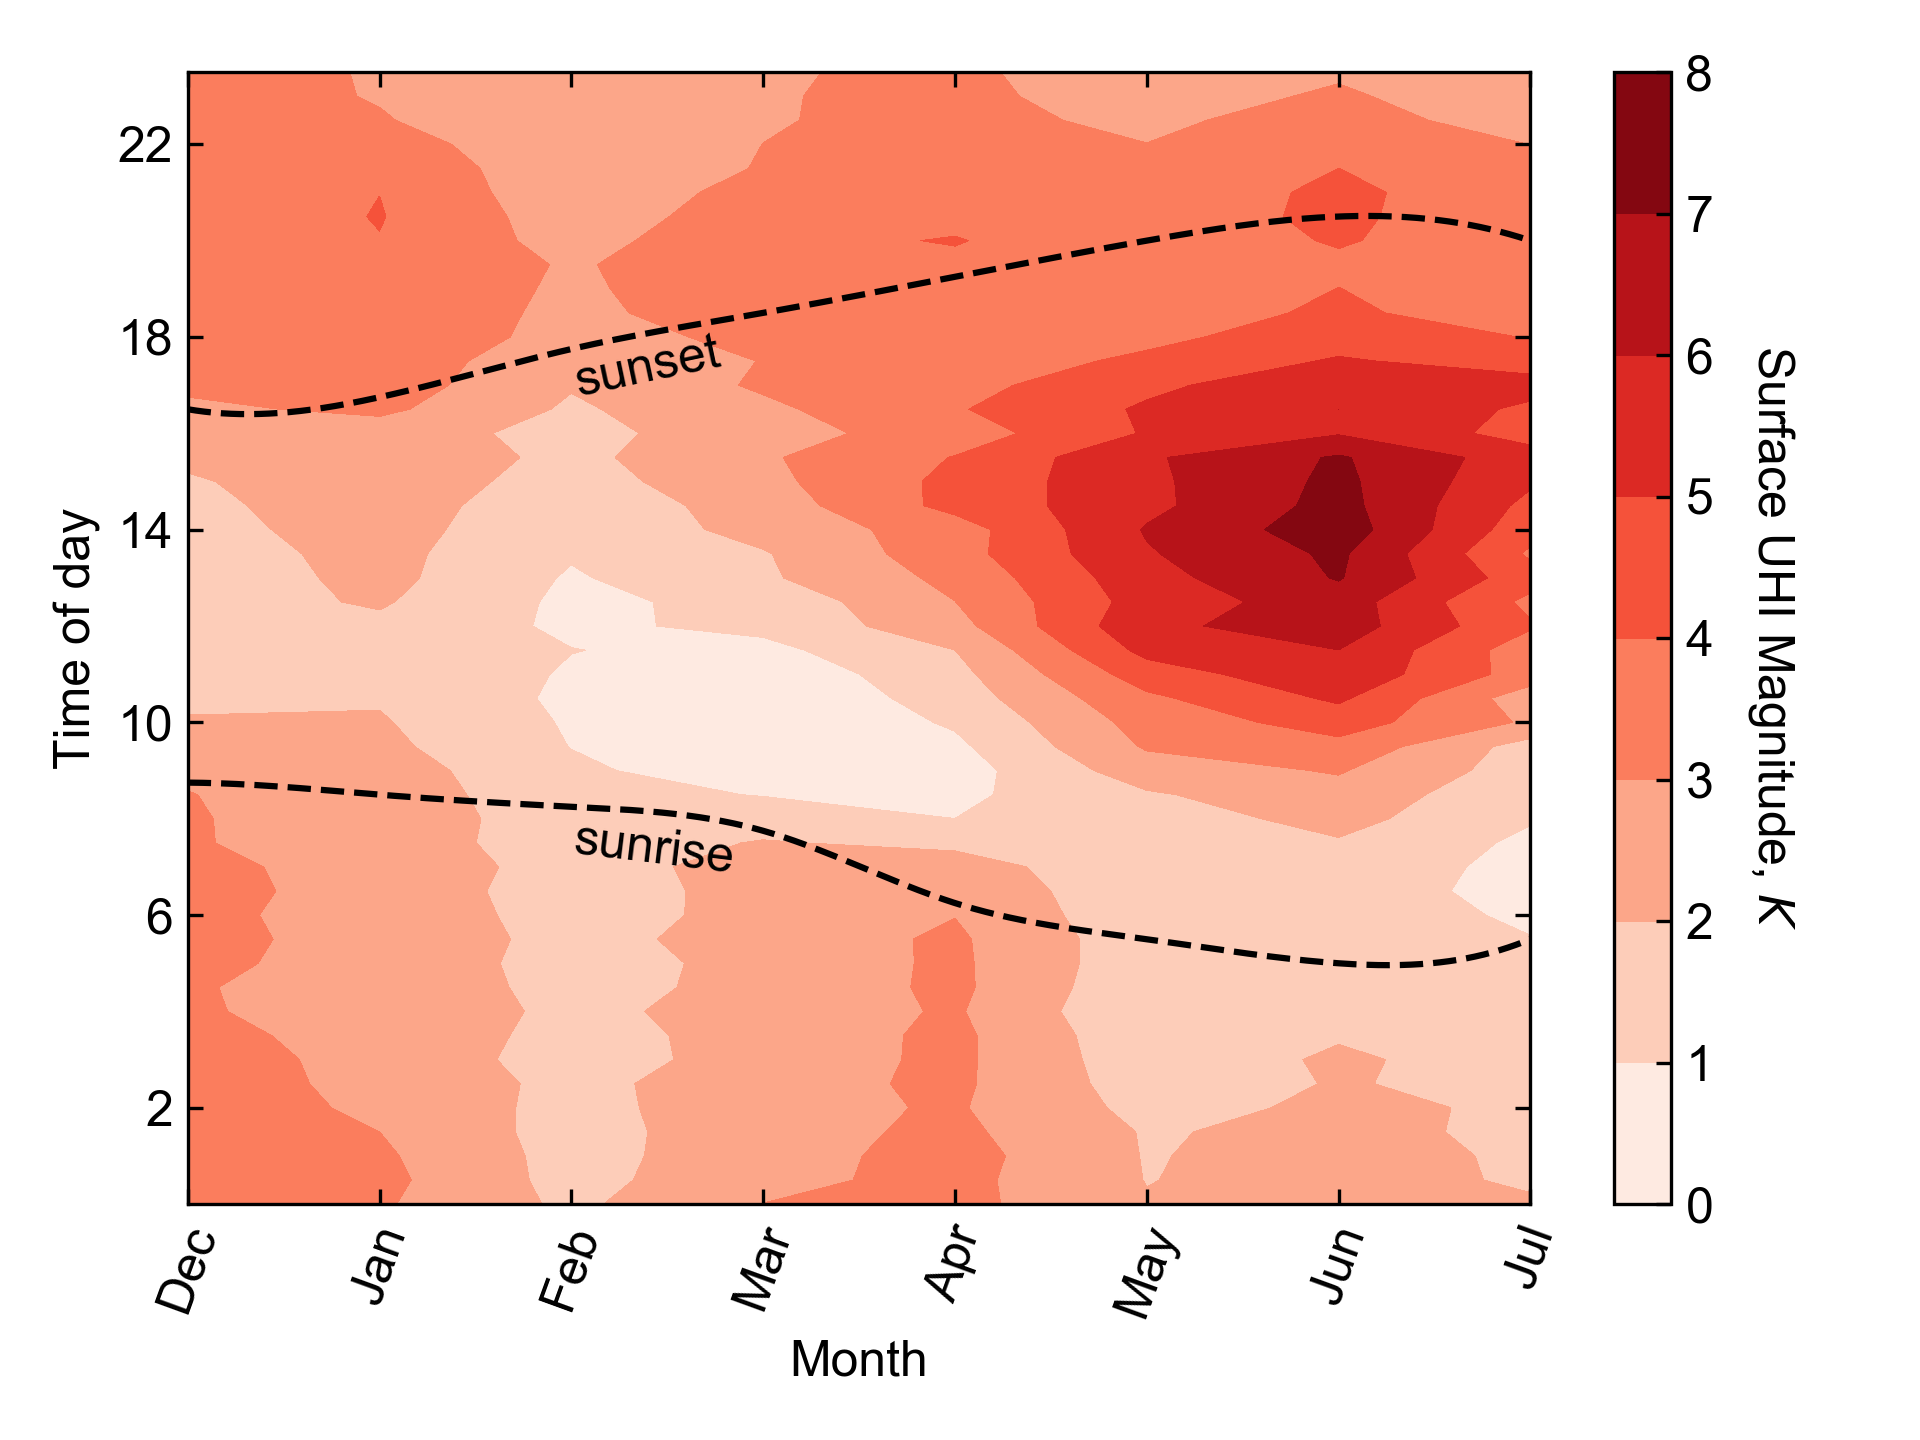
\includegraphics[width=15cm,height=7in,keepaspectratio]{heatsuhi}
	\caption{A heatmap of mean half hourly hemispherical sUHI for each month calculated at 30-minute intervals over the eight month study period.}
	\label{heatsuhi}
\end{figure}

\begin{figure}[H]
	\centering
	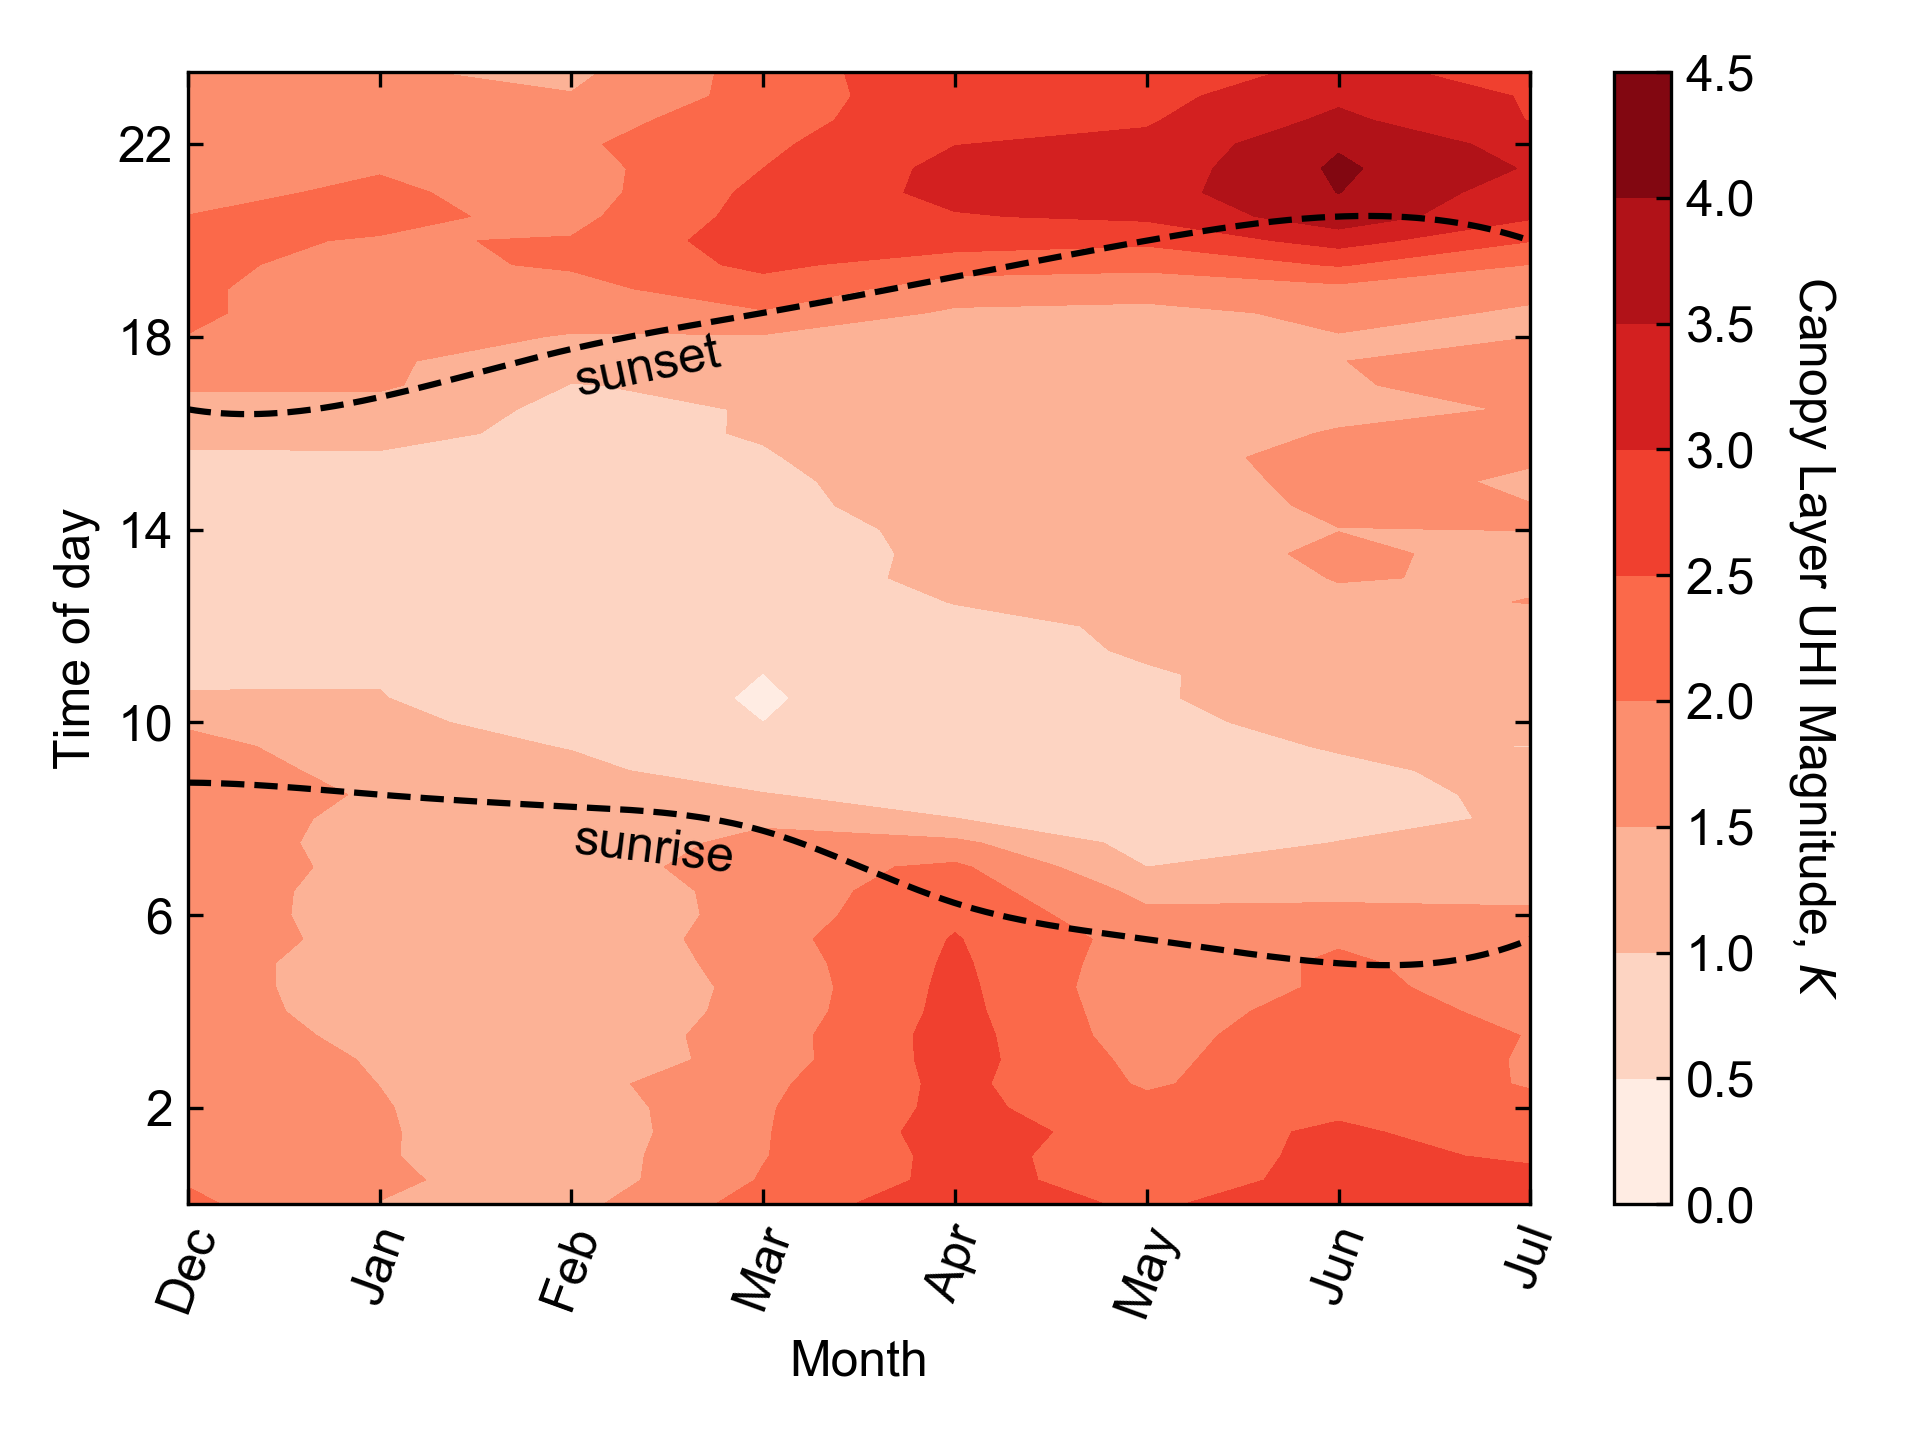
\includegraphics[width=15cm,height=7in,keepaspectratio]{heatatuhi}
	\caption{A heatmap of mean half hourly canopy layer UHI for each month calculated at 30-minute intervals from T\textsubscript{air} measured at approximately 2 \si{\meter} above ground level over the eight month study period.}
	\label{heatcluhi}
\end{figure}

\subsection{The effect of sensor-surface geometry on sUHI}

Figure \ref{bx_suhi_compare} shows sUHI magnitudes calculated from urban T\textsubscript{comp}, T\textsubscript{plan}, and T\textsubscript{hem}. Compared to complete sUHI; nadir and hemispherical views of the surface overestimate sUHI by day and underestimate sUHI by night. sUHI from a nadir view shows the greatest diurnal variance in sUHI, particularly under clear sky 'satellite friendly' conditions. 

\begin{figure}[H]
	\centering
	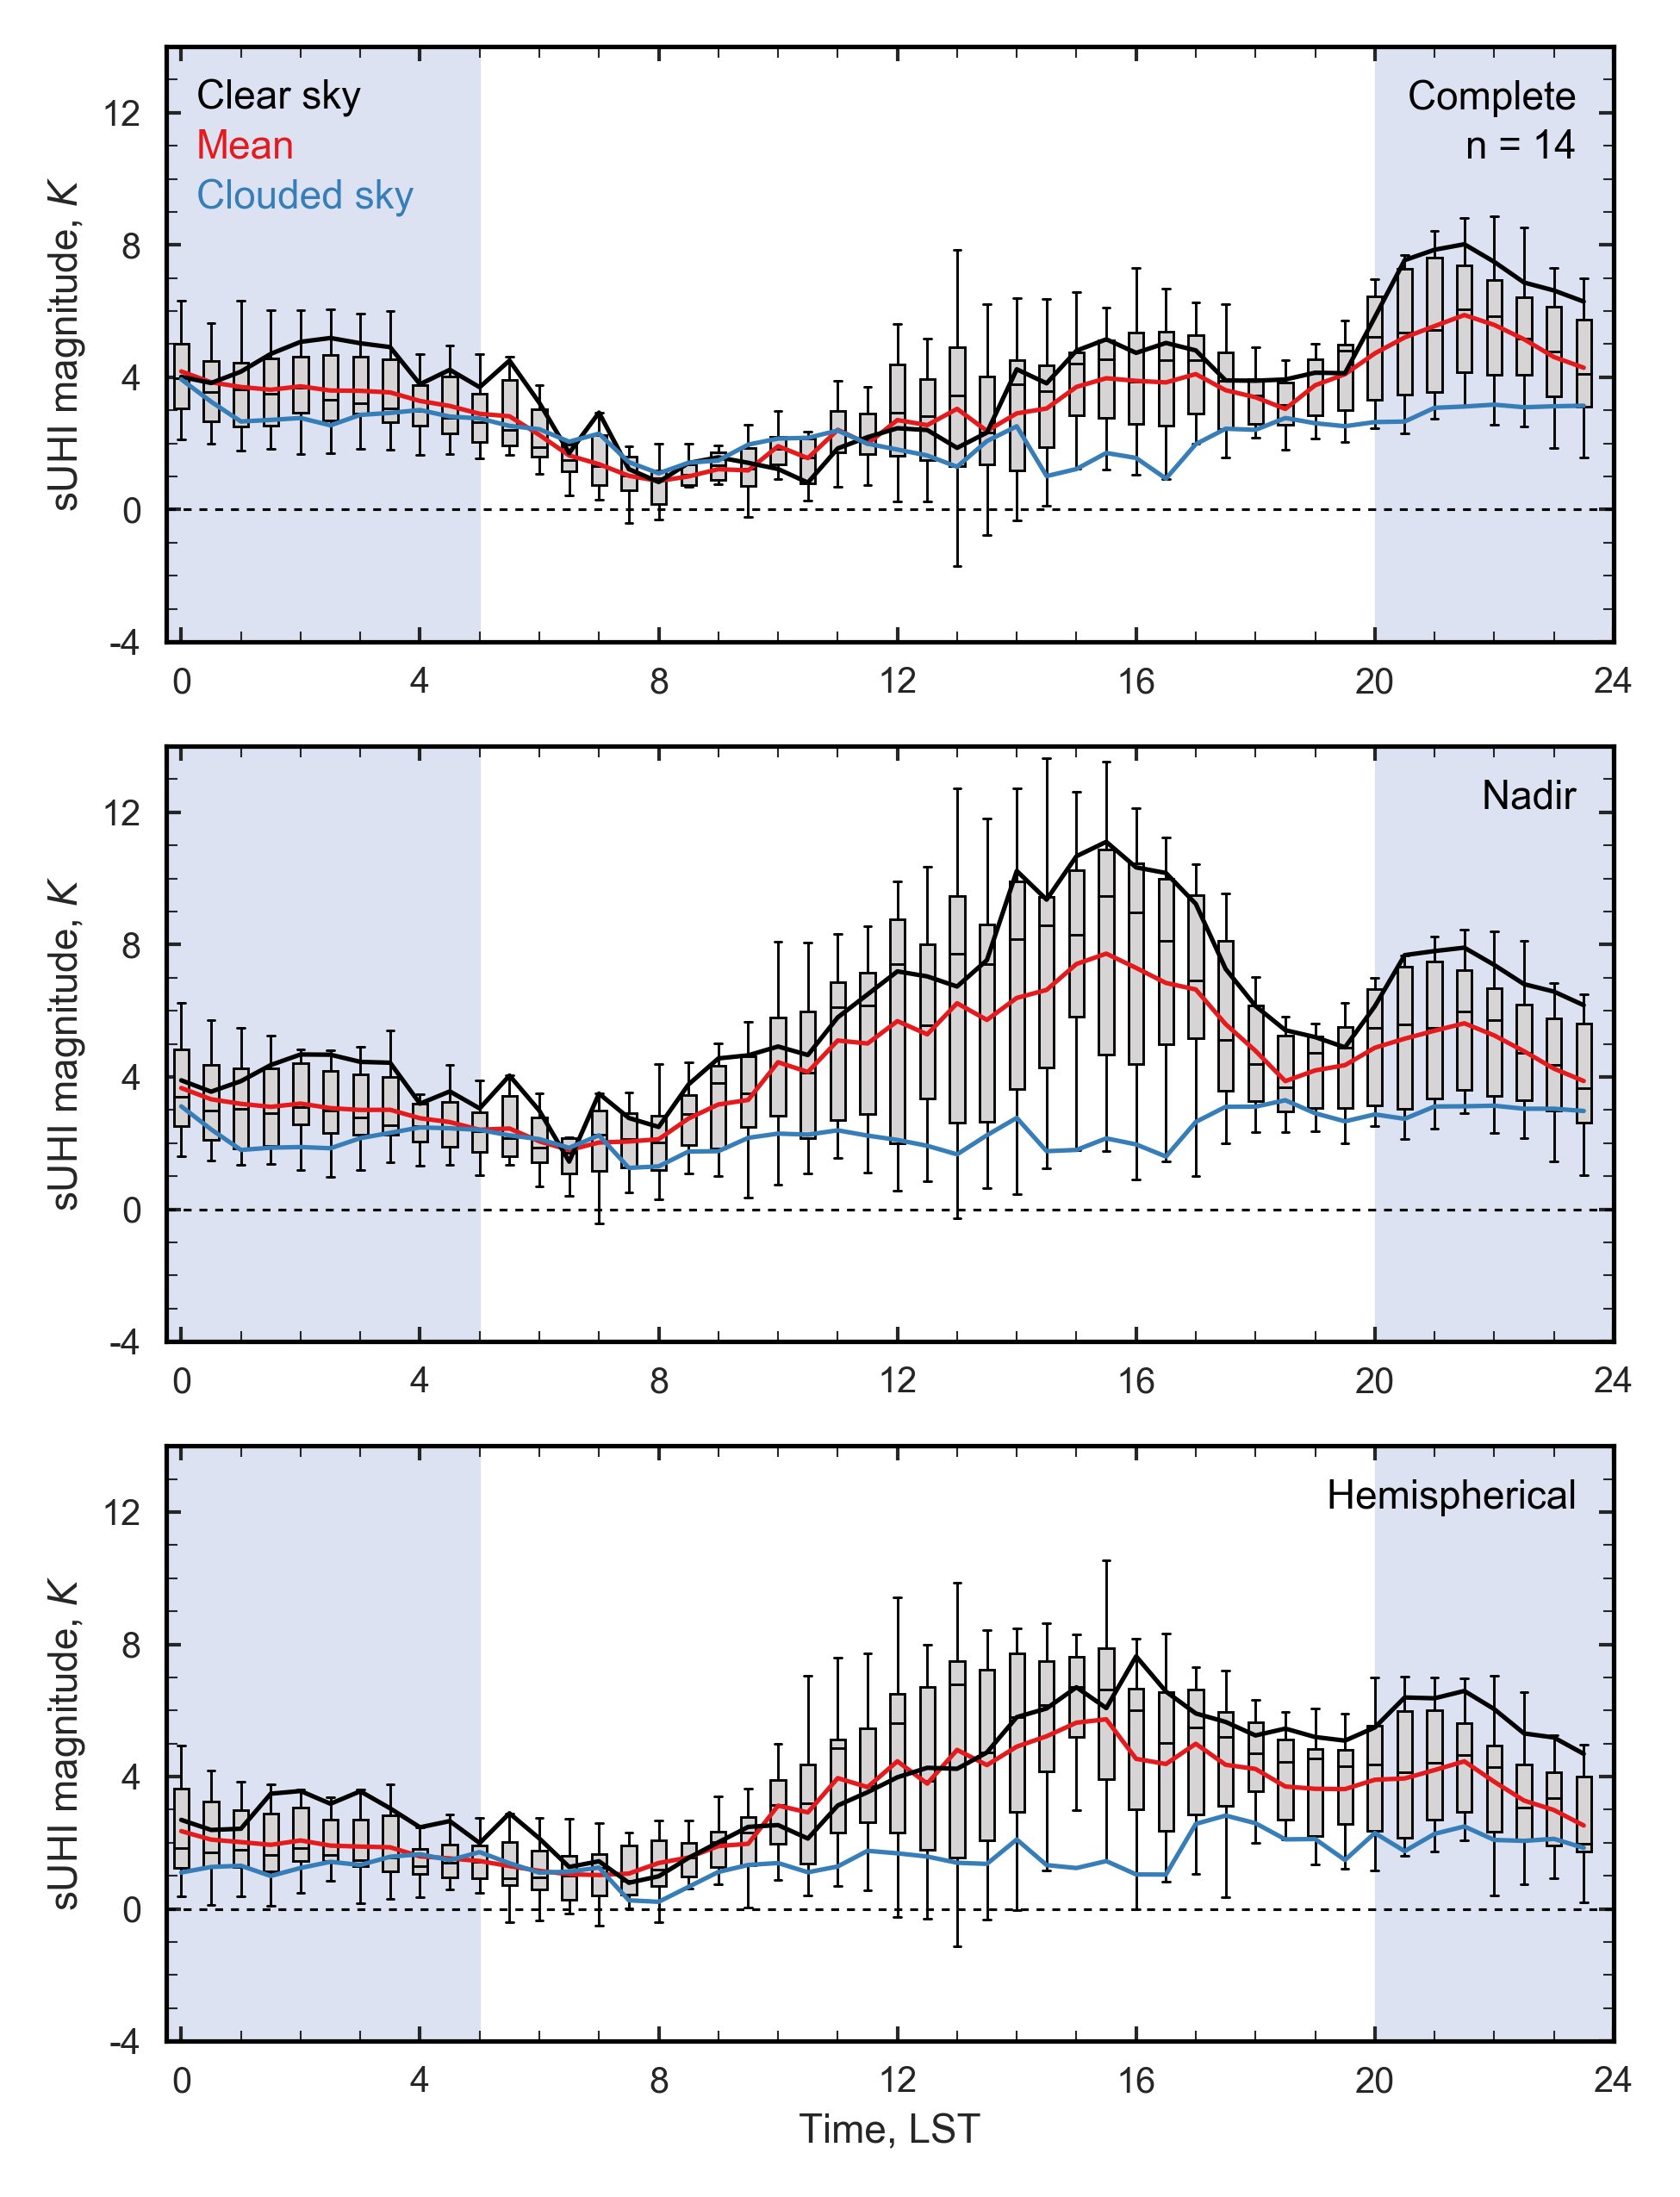
\includegraphics[width=15cm,height=7in,keepaspectratio]{bx_suhi_compare}
	\caption{A comparison of sUHI magnitudes from complete, hemispherical, and nadir remote sensed representations of the Sperrstrasse canyon over the IOP. Each plot includes mean sUHI, as well case days representing sUHI under clear sky and clouded sky conditions.}
	\label{bx_suhi_compare}
\end{figure}

\subsection{The effect of meteorological conditions on sUHI}

Figures \ref{meteo_kdown}, \ref{meteo_hum}, \ref{meteo_wv}, and \ref{meteo_atuhi} show sUHI magnitudes as a function of incoming solar radiation, water vapor content, wind velocity, and clUHI. Winter hours are omitted in Figures \ref{meteo_hum}, and \ref{meteo_wv}, and \ref{meteo_atuhi} as sUHI is small and displays minimal variation in winter. Both winter and nighttime hours are omitted in Figure \ref{meteo_kdown} to examine daytime sUHI under clear sky and clouded sky conditions.

\begin{figure}[H]
	\centering
	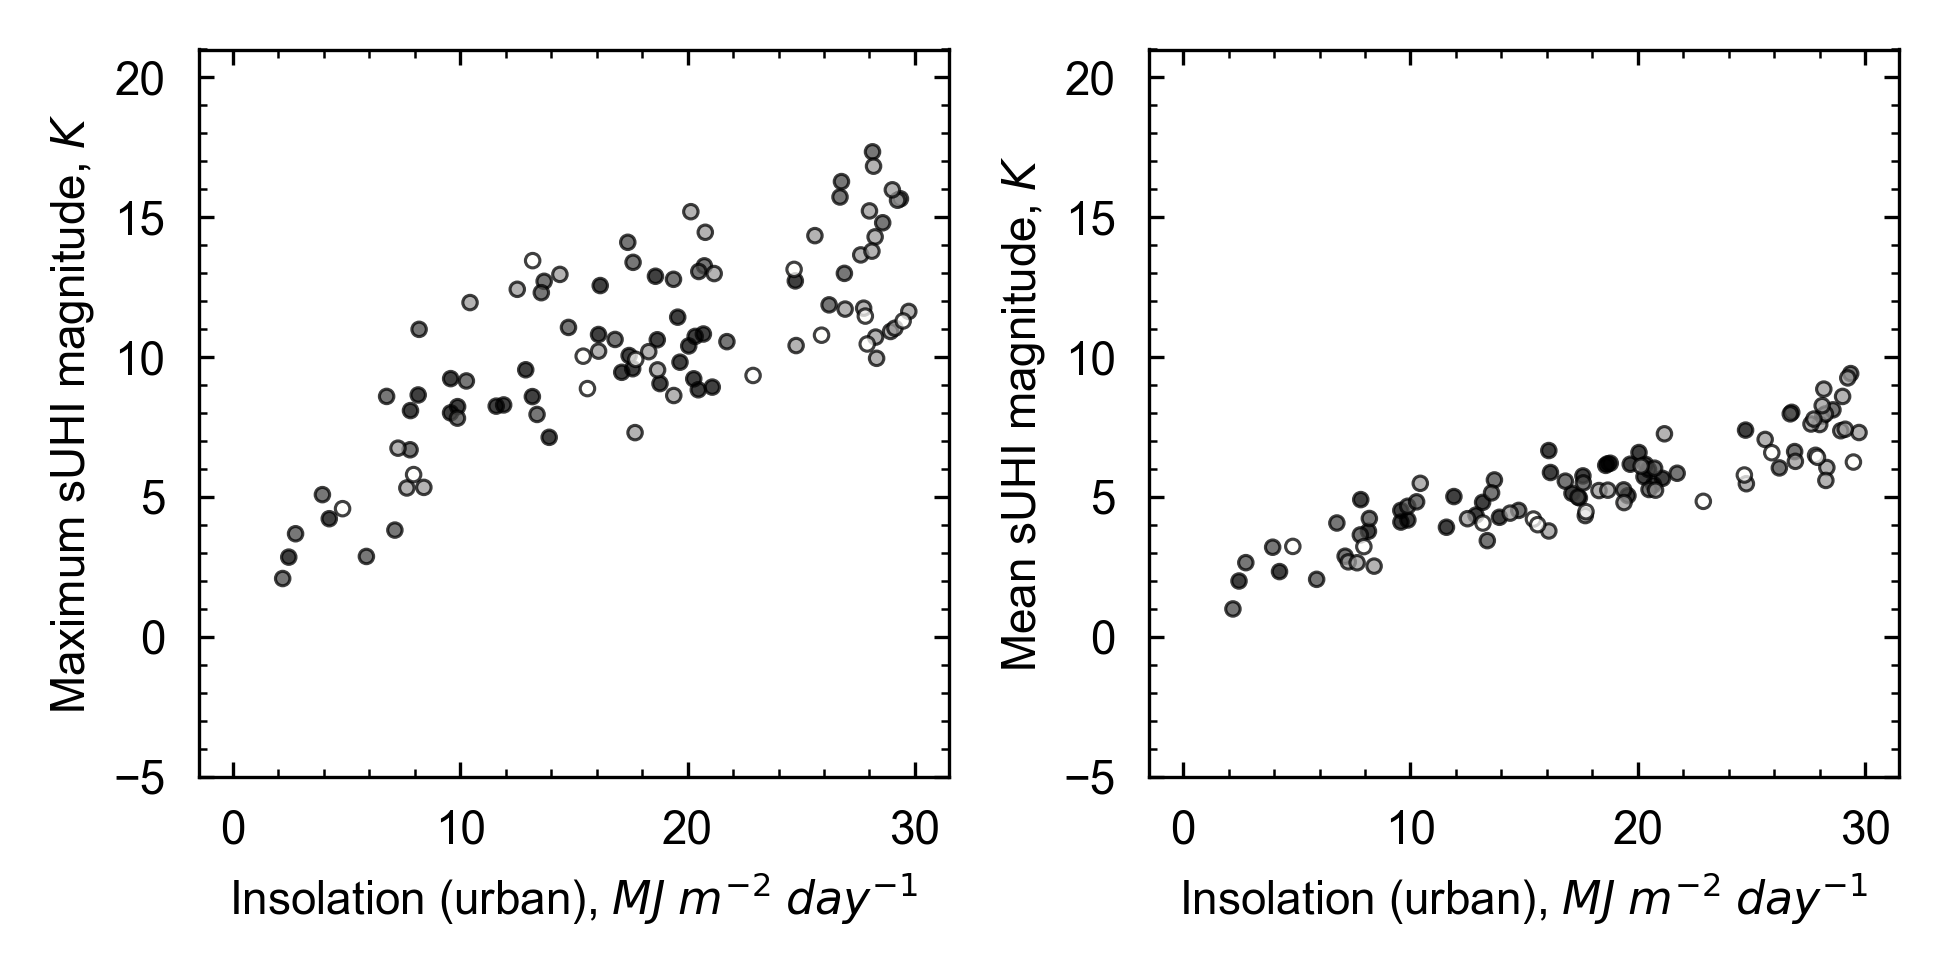
\includegraphics[width=15cm,height=7in,keepaspectratio]{meteo_kdown}
	\caption{sUHI magnitude versus incoming solar radiation binned for clear sky (when the sum of daytime K\textsubscript{down} \textgreater 10000 \si{\watt \per \square \meter})and cloudy sky days (when the sum of daytime K\textsubscript{down} \textless 10000 \si{\watt \per \square \meter})}
	\label{meteo_kdown}
\end{figure}

\begin{figure}[H]
	\centering
	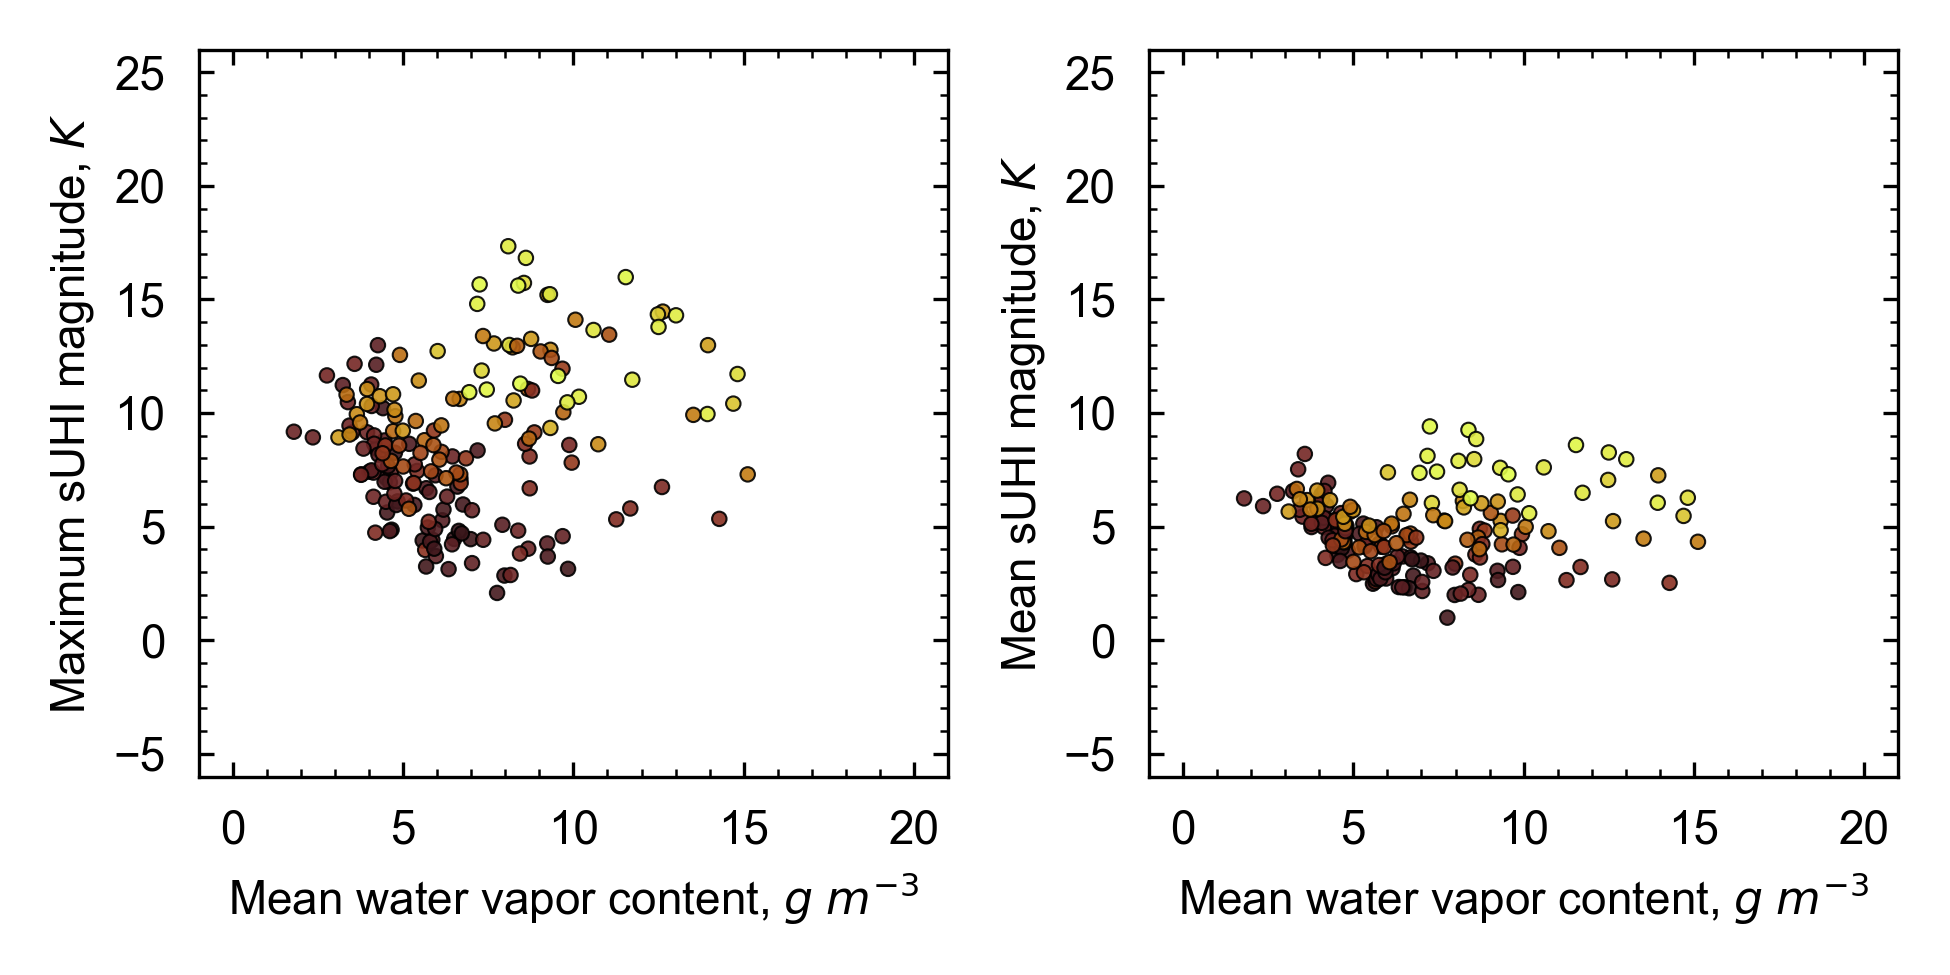
\includegraphics[width=15cm,height=7in,keepaspectratio]{meteo_hum}
	\caption{sUHI magnitude versus atmospheric water vapor content measured at 2 \si{\meter}. Similar patterns are observed when rural water vapor content is substituted.}
	\label{meteo_hum}
\end{figure}

\begin{figure}[H]
	\centering
	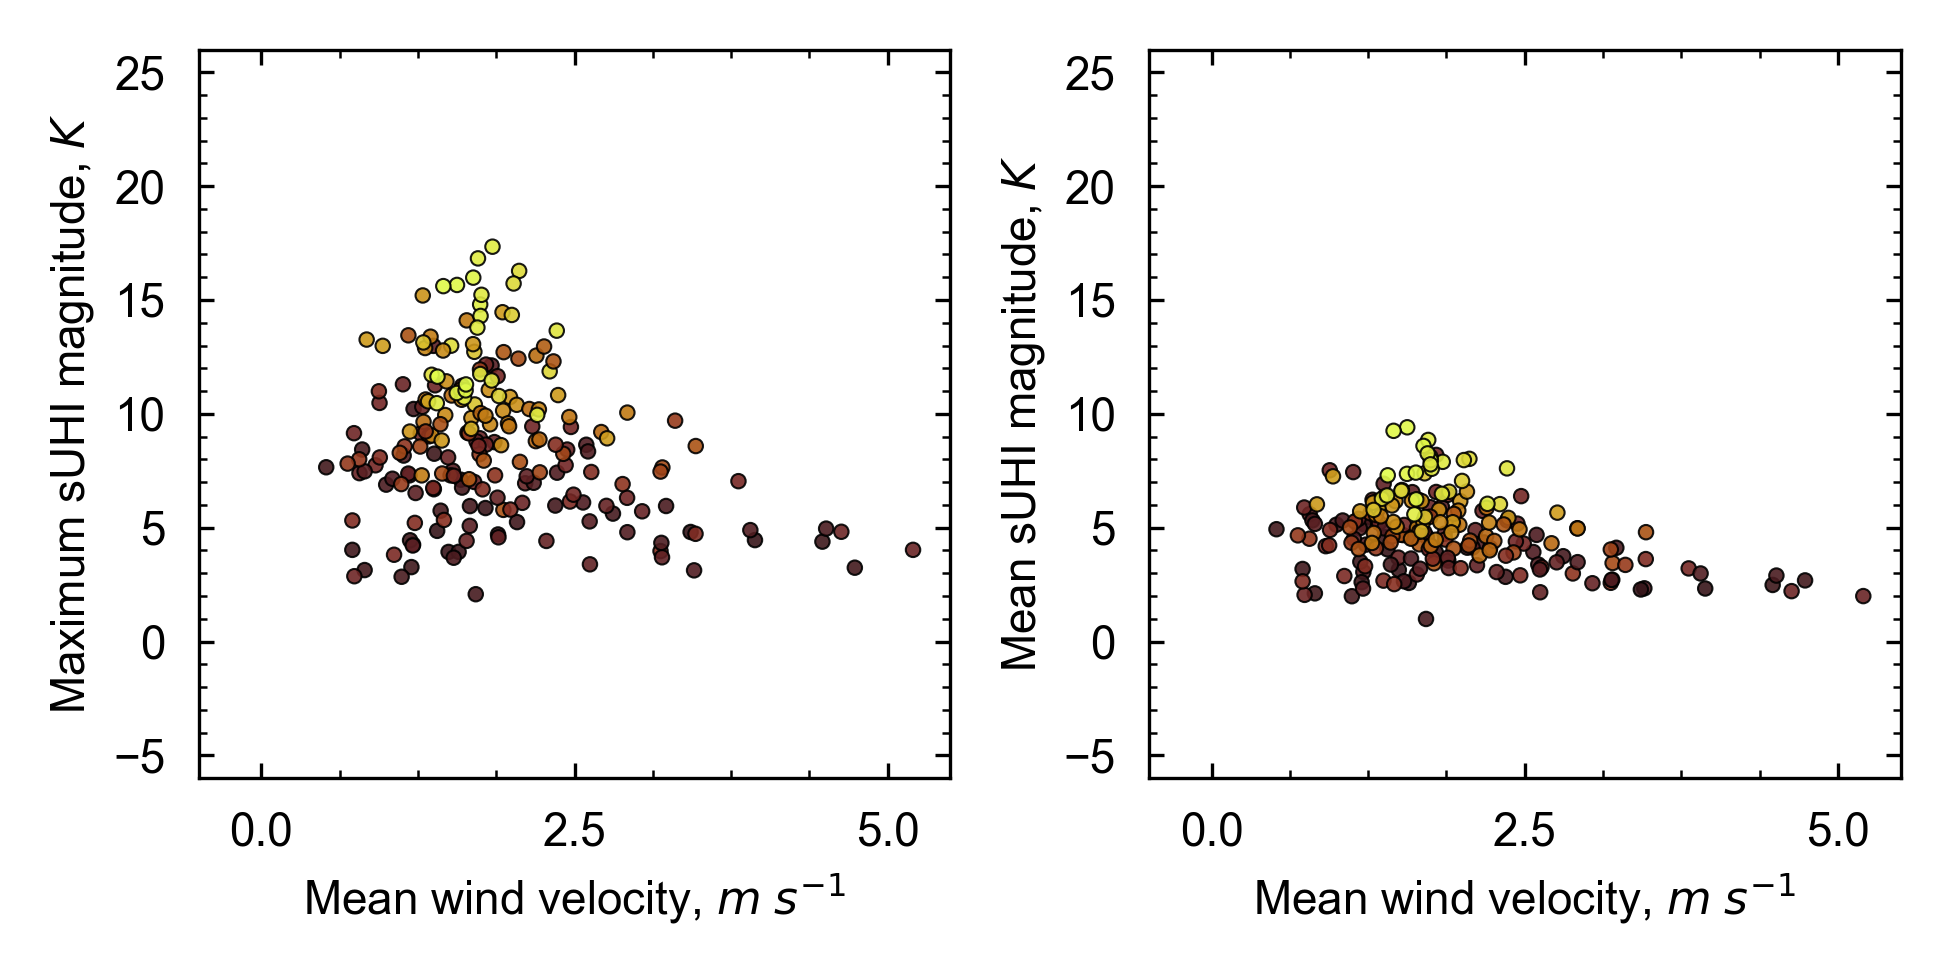
\includegraphics[width=15cm,height=7in,keepaspectratio]{meteo_wv}
	\caption{Bees nest plot}
	\label{meteo_wv}
\end{figure}

\begin{figure}[H]
	\centering
	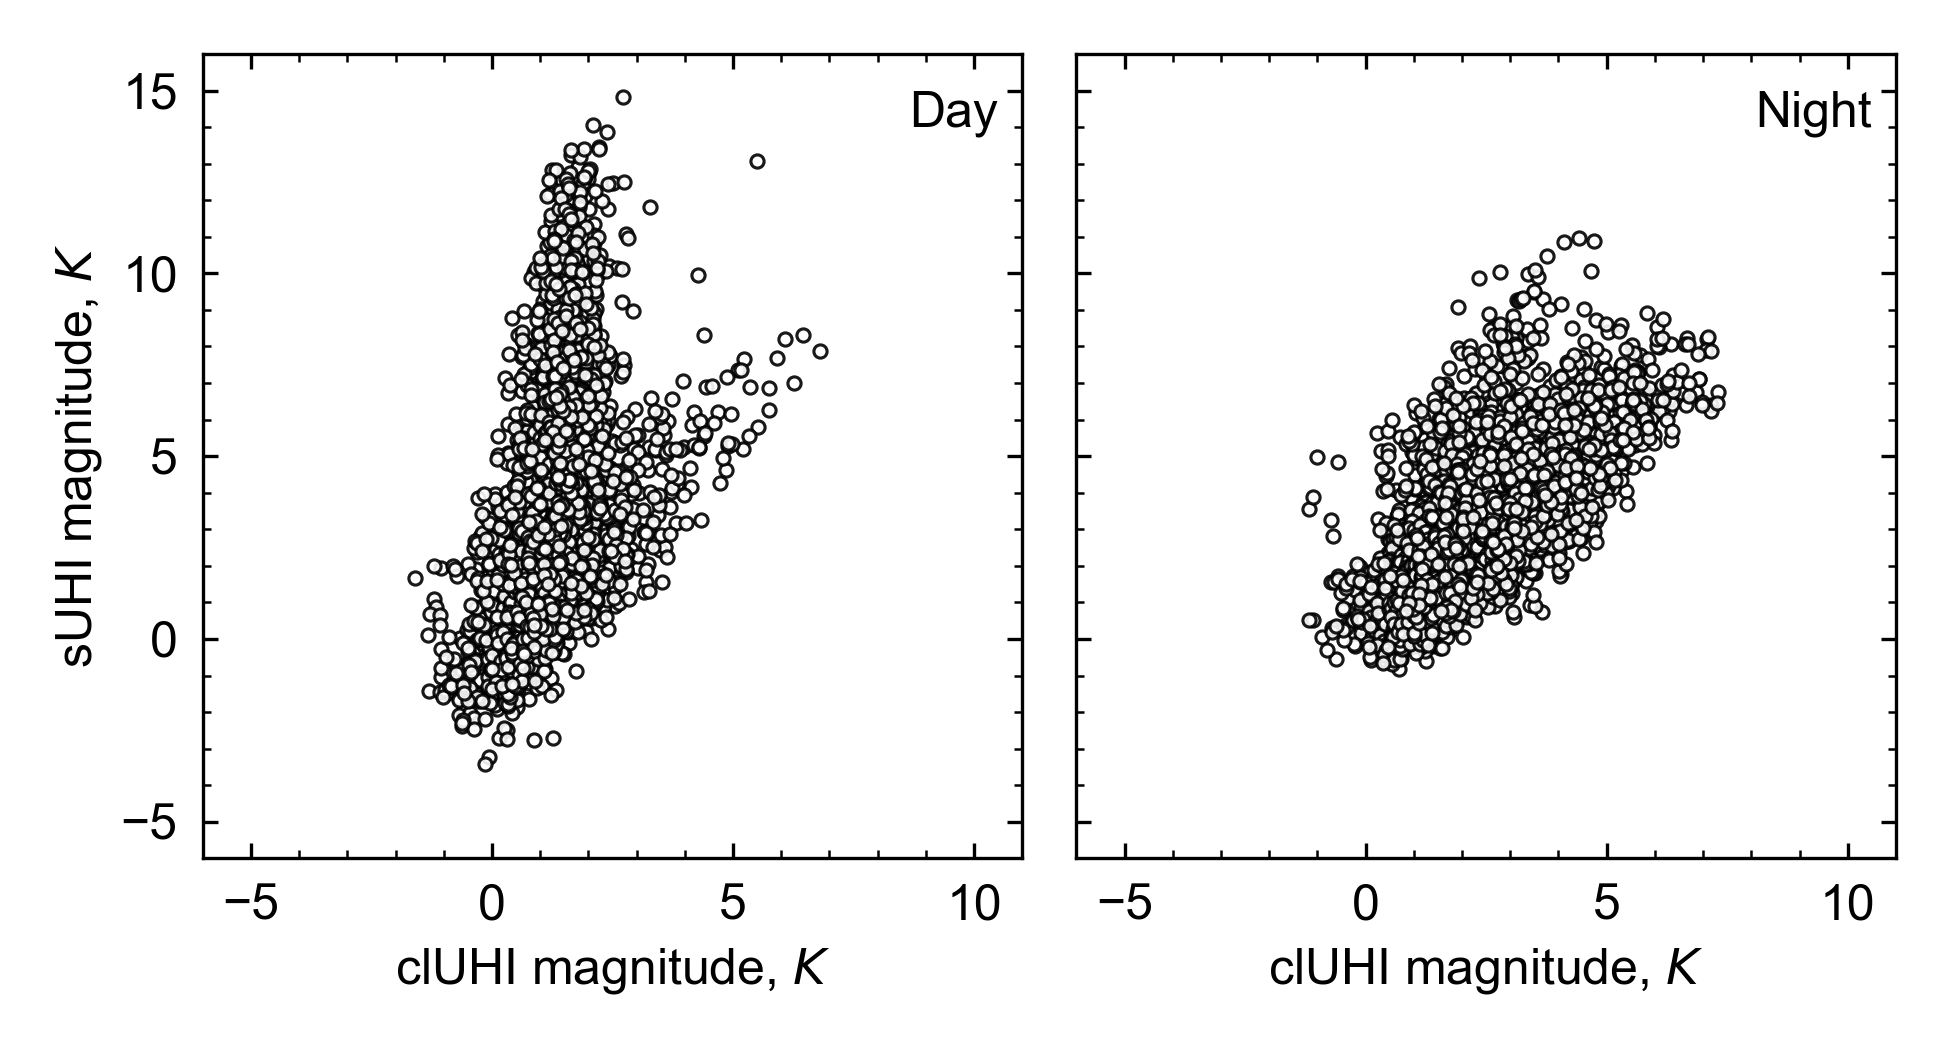
\includegraphics[width=15cm,height=7in,keepaspectratio]{meteo_atuhi}
	\caption{Bees nest plot}
	\label{meteo_atuhi}
\end{figure}

\section{Discussion}

\subsection{Diurnal patterns of sUHI}

sUHI in Basel from complete, nadir, and hemispherical representations of T\textsubscript{surf} displays two diurnal peaks, the first in the late afternoon and a second just after sunset. Clear sky conditions amplify this phenomena. A late afternoon peak in sUHI is likely the result of the urban-rural contrasts in thermal admittance (and by relation, urban-rural soil moisture contrasts). The thermal admittance of many urban surfaces, particularly rooftops, tends to be lower than rural and vegetated environments \cite{Spronken-Smith1998} – particularly in temperate climates where rural soil moisture is largely maintained through summer. Lower urban thermal admittance manifests in a larger diurnal thermal amplitude and thus, greater daytime surface heating and nighttime surface cooling. Nadir and hemispherical views are biased towards low thermal admittance rooftop facets, and thus display large daytime peaks in sUHI.

A second peak in sUHI after sunset is the result of differences in relative cooling rates of urban and rural surfaces. In this case, nighttime sUHI is likely the result of canyon radiation trapping from obstructed canyon sky-view-factors. The second peak sUHI is largest on following clear sky conditions when the potential for significant differentials in urban-rural nocturnal cooling rates is maximized. A second peak is observed across all representations of urban T\textsubscript{surf} but is most apparent in complete and nadir representations of sUHI, which, for the Sperrstrasse site, sample T\textsubscript{road} to a greater extent than the hemispherical view. A weak sUHI is maintained through the nighttime as urban and rural cooling rates reach parity in the hours after sunset \cite{Oke2017}. Minimum sUHI is observed just after sunrise, where sUHI magnitudes are occasionally negative. At low solar angles, shading by 3-dimensional urban geometry suppresses heating rates for a large portion of urban surface area, reducing overall urban heating rates in early morning. As solar angles increase through the morning and more facets experience direct isolation, sUHI develops, with nadir and hemispherical representations displaying more rapid intensification than complete sUHI from a bias towards low thermal admittance and directly sunlit rooftop surfaces.

\subsection{Seasonal patterns of sUHI}

Hemispherical sUHI displays significant seasonality, both in terms of its diurnal pattern and overall magnitude. Seasonal variance in sUHI is greatest by day, where large seasonal contrasts in cloud cover frequency and solar angle exert strong control on daytime heating rates and sUHI development. Peak sUHI occurs near the summer solstice, when days are longest and isolation on clear sky days is most intense. In winter, daytime sUHI is suppressed from a lower solar input and frequent cloud cover. This shifts and weakens peak sUHI in winter to shortly after sunset. Nighttime sUHI is relatively consistent across seasons, largely a product of contrasts in urban-rural cooling rates just after sunset resulting from radiation trapping by canyon geometry. Similar patterns are observed in seasonal variance of canopy layer UHI, albeit concentrated at different times of day. 

In contrast to sUHI, clUHI is greatest just after sunset and is strongly controlled by sunset/sunrise timing. Peak clUHI occurs just after sunset across seasons, differing only in terms of magnitude, with a larger peak clUHI in summer. However, in this study, it should be note that summertime clUHI magnitudes in the hours just after sunset are slightly higher than expected \cite{Runnalls2000} – possibly the result of cold air draining from hilly terrain west of the rural site. Seasonality in clUHI results from seasonal contrasts in cloud cover frequency. Increased wintertime cloud cover reduces radiative losses by the canyon air volume after sunset, suppressing mean wintertime clUHI magnitudes. Daytime clUHI is consistently small across all seasons. Thus, although sUHI and clUHI are controlled by similar climatic controls and have a similar micro meteorological genesis, they do not display the same seasonal patterns. Thus, \textit{a surface urban heat island is not simply a stronger, more pronounced, canopy layer urban heat island.}

\subsection{Sensor-surface-sun geometries and sUHI}

Sensor-surface geometry exerts significant influence on observed sUHI magnitudes. By undersampling vertical and sloped urban surfaces and oversampling low thermal admittance fabric materials, nadir sUHI overestimates mean afternoon complete sUHI by 3.41 \si{\kelvin} and up to 5.96 \si{\kelvin} under clear sky “satellite friendly” conditions. Thus, peak nadir sUHI overestimates the peak 'true' complete sUHI by nearly double under clear sky conditions. As clear sky conditions are the only conditions under which satellite TIR remote sensors can operate, and make up a large fraction of the urban T\textsubscript{surf} literature, these biases cannot be ignored. By sampling the urban surface in 3-dimensions, hemispherical sUHI yields a much smaller mean daytime overestimation (0.54 \si{\kelvin}), particularly under clear sky conditions (0.93 \si{\kelvin}), providing a more geometrically representative depiction of complete urban T\textsubscript{surf} and sUHI, in addition to allowing for time-continuous analysis. Cloud cover suppresses the influence of sensor-surface geometry on remote sensed sUHI by reducing microscale geometric and spatiotemporal contrasts in urban T\textsubscript{surf}, resulting in less facet-scale heterogeneity in urban T\textsubscript{surf} and reducing the overall magnitude of sUHI.


\subsection{Meteorological controls on sUHI}

sUHI is highly dependent on meteorological conditions, which account for much of the variation in daytime sUHI magnitudes. Conditions that foster the largest microscale contrasts in urban T\textsubscript{surf} also entail the largest sUHI magnitudes. Contra, conditions that suppress microscale contrasts in T\textsubscript{surf} show similarly reduced sUHI magnitudes. As such, incoming shortwave radiation and wind velocity display positive and negative relationships with sUHI magnitudes respectively. Under clear sky conditions, strong solar heating of the surfaec combined with differences in urban and rural thermal properties fosters the development of large daytime urban-rural thermal contrasts. Thus, sUHI\textsubscript{max} coincides with insolation\textsubscript{max}. Under cloudy conditions, decreased direct solar heating of the surface suppresses the development of urban-rural thermal contrasts, resulting in a reduced sUHI. $\Delta$T\textsubscript{hem, r - air} has a similar positive effect on sUHI, owing to its dependence on solar insolation. 

As was found with correction magnitudes in Chapter \ref{paper1}, sUHI magnitudes are not strongly correlated with water vapor content as, in the absence of fog, humidity near the surface does not strongly influence surface heating or cooling rates in and of itself. Atmospheric transmittance of longwave radiation decreases sharply with small increases in water vapor when the atmosphere is relatively dry - shown in Figure \ref{humtest} - with decreasing variation in atmospheric transmittance as water vapor content increases from zero. Therefore, typical variations in urban and rural humidities have little effect on the fraction of outgoing available for heating of the canopy layer air volume through absorption of outgoing longwave radiation and for heating of the surface by atmospheric emission towards the surface. As a result, water vapor content has little effect on sUHI. Wind velocity displays a strong negative relationship with sUHI. sUHI is greatest under calm winds when near-surface mixing is minimal, fostering strong microscale and urban-rural contrasts in T\textsubscript{surf}. As wind velocity increases, sUHI is suppressed from increased turbulent heat losses.

\begin{table}[H]
	\centering
	\caption{A summary of the relationship between sUHI, meteorological variables, and clUHI.}
	\label{meteo_cont}
	\begin{tabular}{lc}
		\toprule 
		An increase in $x$, has a/an... & $y$ effect on sUHI magnitude. \\
		\midrule
		$\Delta$T\textsubscript{hem, r - air} &\textit{increasing} \\
		&\\
		T\textsubscript{hem, r} & \textit{increasing} \\
		&\\
		T\textsubscript{air} & \textit{increasing} \\
		&\\
		clUHI &\textit{increasing} \\
		&\\
		Incoming solar radiation & \textit{increasing}  \\
		& \\
		& \\
		Water vapor content & \textit{negligible} \\
	 	&\\
		Wind velocity &\textit{decreasing} \\
		\bottomrule
	\end{tabular} 
\end{table}

clUHI and sUHI develop at different times of day and, thus, have a complex diurnal relationship. By day, variation in clUHI is minimal and shows a weak positive correlation with sUHI. By night, clUHI shows greater variation and a stronger positive relationship with sUHI. Increasing sUHI with clUHI is largest on clear sky nights when urban-rural contrasts in air and surface cooling rates are strongest. This results in similar sUHI and clUHI development in the hours after sunset under clear sky conditions. 

\section{Conclusion}

This chapter presents the results of a time-continuous eight month climatological analysis of the surface urban heat island effect in Basel, Switzerland derived using the method presented in Chapter \ref{paper1}. Hemispherical sUHI magnitudes show significant seasonal and diurnal variation and are largest in summer months during the late afternoon during which solar heating of the surface is most intense, forcing the development of strong microscale and urban-rural contrasts in T\textsubscript{surf}. Variation in afternoon sUHI is largely dependent on incoming solar radiation, which displays a strong positive relationship with sUHI magnitudes. Similarly, sUHI displays positive relationships with $\Delta$T\textsubscript{hem, r} and nighttime clUHI and a negative relationship with wind velocity. In the winter months, a lower overall solar input and increased cloud cover frequency suppresses daytime sUHI development day-to-day variation in sUHI.

 To elucidate the effect of surface-sensor geometry on remote sensed sUHI patterns, sUHI was calculated using weighted facet T\textsubscript{surf} to compute complete and plan representations of sUHI against sUHI calculated from T\textsubscript{hem, r}


%----------------------------------------------------------------------
% END MATERIAL
%----------------------------------------------------------------------

% B I B L I O G R A P H Y
% -----------------------

% The following statement selects the style to use for references.  It controls the sort order of the entries in the bibliography and also the formatting for the in-text labels.
\bibliographystyle{apalike}
% This specifies the location of the file containing the bibliographic information.  
% It assumes you're using BibTeX (if not, why not?).
\cleardoublepage % This is needed if the book class is used, to place the anchor in the correct page,
% because the bibliography will start on its own page.
% Use \clearpage instead if the document class uses the "oneside" argument
\phantomsection  % With hyperref package, enables hyperlinking from the table of contents to bibliography             
% The following statement causes the title "References" to be used for the bibliography section:
\renewcommand*{\bibname}{References}

% Add the References to the Table of Contents
\addcontentsline{toc}{chapter}{\textbf{References}}

\bibliography{library}
% Tip 5: You can create multiple .bib files to organize your references. 
% Just list them all in the \bibliogaphy command, separated by commas (no spaces).

% The following statement causes the specified references to be added to the bibliography% even if they were not 
% cited in the text. The asterisk is a wildcard that causes all entries in the bibliographic database to be included (optional).
% The \appendix statement indicates the beginning of the appendices.
\appendix
% Add a title page before the appendices and a line in the Table of Contents

\end{document}
